\documentclass[openany]{tietreport}

\usepackage{graphicx}
\usepackage{booktabs}
\usepackage{tabularx}
\usepackage{xltabular}
\usepackage{array}
\usepackage{float}
\raggedbottom
\newcolumntype{Y}{>{\raggedright\arraybackslash}X}
\setlength{\headheight}{15pt}

% ---- layout: symmetric margins and the same running header on every page
\geometry{inner=1.2in, outer=1.2in, top=1.5in, bottom=1in, headsep=0.3in}
\fancyhf{}
\fancyhead[L]{\small UCS503 Software Engineering Lab \quad|\quad hackViz}
\fancyhead[R]{\small\thepage}

% ---- captions, lists, tables, floats
\usepackage[font=small, labelfont=bf, labelsep=period, justification=centering, skip=6pt]{caption}
\captionsetup[table]{position=top, skip=4pt}
\usepackage{enumitem}
\setlist{itemsep=3pt, topsep=4pt, parsep=0pt, leftmargin=1.6em}
\setlist[enumerate]{leftmargin=1.9em}
\renewcommand{\arraystretch}{1.25}
\setlength{\parskip}{2pt}
\setlength{\emergencystretch}{3em}
\makeatletter
\let\cleardoublepage\clearpage
\setlength{\@fptop}{0pt}
\setlength{\@fpsep}{14pt}
\setlength{\@fpbot}{0pt plus 1fil}
\makeatother
\renewcommand{\topfraction}{0.9}
\renewcommand{\bottomfraction}{0.8}
\renewcommand{\textfraction}{0.07}
\renewcommand{\floatpagefraction}{0.75}

% ---- story card: {ID}{story}{priority}{points}{acceptance}{status}
\newcommand{\storycard}[6]{%
  \fbox{\parbox[t][5.0cm][t]{0.455\linewidth}{\small
    \textbf{#1}\hfill Priority: #3 \;|\; Points: #4\par
    \vspace{-2pt}\rule{\linewidth}{0.4pt}\par\vspace{2pt}
    #2\par\vspace{4pt}
    \textbf{Acceptance criteria:} #5\par\vspace{4pt}
    \textbf{Status:} #6}}}

% ---- use case template table
\newcommand{\uctable}[9]{%
\begin{table}[H]
\centering
\small
\caption{Use case template #1: #2.}
\begin{tabularx}{\linewidth}{@{}>{\bfseries}p{3.3cm}Y@{}}
\toprule
1. Use Case Title & #2 \\
2. Use Case Id & #1 \\
3. Actors (type) & #3 \\
4. Description & #4 \\
5. Pre Conditions & #5 \\
6. Typical Course of Events & #6 \\
7. Alternate Flow & #7 \\
8. Exceptional Flow & #8 \\
9. Post Conditions & #9 \\
\bottomrule
\end{tabularx}
\end{table}}

% ---- edit these two values if needed
\newcommand{\GroupNo}{3C25}
\newcommand{\MonthYear}{November 2026}

\begin{document}

% ===================================================== COVER / TITLE PAGE
\begin{titlepage}
\thispagestyle{empty}
\begin{flushright}\small\bfseries UCS503- Software Engineering Lab\end{flushright}
\vspace*{0.6cm}
\begin{center}
{\LARGE\bfseries hackViz: Explainable Insider-Threat Detection\par}
\vspace{0.3cm}
{\large Role-aware anomaly assessment of employee activity\\ with a local Transformer language model\par}
\vspace{0.9cm}
{\large\bfseries UCS 503 Software Engineering Project Report\par}
\vspace{0.25cm}
{\large\bfseries END-Semester Evaluation\par}
\vspace{1.1cm}
{\large\bfseries Submitted by:\par}
\vspace{0.3cm}
{\large\bfseries
(1024030380) Shreshth Garg\\[4pt]
(1024030954) Geetansh Bansal\\[4pt]
(1024030383) Lakshit Goyal\par}
\vspace{0.8cm}
{\large\bfseries BE Third Year, CSE\par}
\vspace{0.2cm}
{\large\bfseries Group No: \GroupNo\par}
\vspace{0.8cm}
{\large\bfseries Submitted to:\par}
\vspace{0.2cm}
{\large Dr. Stuti Chug\par}
\vspace{0.9cm}
\IfFileExists{figures/tiet_logo.png}{\includegraphics[width=3.2cm]{figures/tiet_logo.png}\par\vspace{0.6cm}}{\vspace{1.2cm}}
{\bfseries Computer Science and Engineering Department\par}
\vspace{0.15cm}
{\bfseries TIET, Patiala\par}
\vspace{0.15cm}
{\bfseries \MonthYear\par}
\end{center}
\end{titlepage}

\tableofcontents

% ===================================================== 1. PROJECT SELECTION PHASE
\chapter{Project Selection Phase}

\section{Software Bid}

Table~\ref{tab:bid} is the team's bid for the project: what will be built, for whom, with which
resources and in what time.

\begin{table}[H]
\centering
\small
\caption{Software bid.}
\label{tab:bid}
\begin{tabularx}{\linewidth}{@{}>{\bfseries}p{3.0cm}Y@{}}
\toprule
Project title & hackViz: Explainable Insider-Threat Detection \\
Team & Shreshth Garg, Geetansh Bansal, Lakshit Goyal (BE Third Year, CSE) \\
Intended users & Security analysts and system administrators of an organisation; employees whose
  browser activity is monitored with consent \\
Problem & Detecting insider threats and explaining each alert (Section~\ref{sec:background}) \\
Proposed solution & Explainable detection platform built around a local Transformer model
  (Section~\ref{sec:arch}) \\
Deliverables & Chrome extension; FastAPI backend with PostgreSQL; analysis worker with the local model;
  React dashboard; reproducible CERT-style dataset of ten employees; automated tests; documentation \\
Technology & Python 3.12, FastAPI, SQLAlchemy, PostgreSQL 16, Ollama with Qwen2.5-3B, React 18 with Vite,
  Chrome Manifest V3, pytest, Puppeteer \\
Hardware & One Windows laptop, 16\,GB RAM, CPU only (no GPU) \\
Cost & No licence or cloud cost: all tools are free and open source and the model runs locally \\
Duration & 11 weeks (Table~\ref{tab:plan}) \\
Main risks & Slow inference on a CPU; the model citing records that do not exist; privacy of monitored
  employees. Mitigations: background analysis, evidence verification, metadata-only collection with
  consent. \\
\bottomrule
\end{tabularx}
\end{table}

\begin{table}[H]
\centering
\small
\caption{Weekly plan followed by the team (from the project journal).}
\label{tab:plan}
\begin{tabularx}{\linewidth}{@{}lYY@{}}
\toprule
\textbf{Week} & \textbf{Work} & \textbf{Output} \\
\midrule
1 & Project setup, search for a suitable dataset & CERT insider-threat dataset chosen \\
2 & Novelty requirement, DeepLog literature review & Problem framing, related work \\
3 & CERT exploratory data analysis & Understanding of event types and volumes \\
4 & Preprocessing and event unification design & Common event schema \\
5 & Temporal engine: how to feed behaviour to a model & Baseline and analysis-window design \\
6 & Handling e-mail and file content & Metadata-only decision \\
7 & Choosing the architecture & Local LLM with validation \\
8 & Users for mock demonstration data & Ten fictional employees, seeded dataset \\
9 & Implementation: backend, model pipeline, extension & Working end-to-end system \\
10 & Evaluating performance & Test suite, timing measurements \\
11 & Integration, testing and documentation & 54 tests passing, report \\
\bottomrule
\end{tabularx}
\end{table}

\section{Project Overview}

\subsection{Background and Problem}
\label{sec:background}

Insider threats are security incidents caused by people who already have legitimate access to an
organisation's systems~\cite{cappelli2012cert,homoliak2019insight}. Copying confidential files uses the
same credentials and tools as normal work, so what matters is the \emph{context}: who acted, whether it
fits their role and history, and how actions combine. Rule-based SIEM tools produce many false
positives, and behaviour-based detectors such as Isolation Forest~\cite{liu2008isolation} or
DeepLog~\cite{du2017deeplog} output a score that does not explain itself~\cite{doshivelez2017towards}.
hackViz addresses this with a Transformer-based language
model~\cite{vaswani2017attention,qwen2024qwen25}, run locally through Ollama~\cite{ollama}, whose
explanations an analyst can check against real records.

\subsection{Objectives}

\begin{enumerate}
  \item Generate a reproducible, fictional CERT-style dataset of ten employees in different
    roles~\cite{glasser2013bridging}.
  \item Build a Chrome extension that collects navigation and download metadata only after consent and
    stops when disconnected.
  \item Store and validate all activity in PostgreSQL through a FastAPI backend.
  \item Produce explainable assessments with a local Transformer model in which every cited evidence ID
    is verified.
  \item Present results on an analyst dashboard and verify the whole workflow with real browser activity.
\end{enumerate}

\subsection{Scope}
\label{sec:scope}

In scope: activity collection and ingestion, per-employee analysis, explainable risk assessment,
analyst review with evidence drill-down, CSV export and system monitoring. Out of scope: automatic
blocking of users. Not yet implemented: login and roles, analyst confirm/dismiss feedback, audit
logging, and the Transformer decoder for sequence scoring.

\subsection{System Architecture}
\label{sec:arch}

hackViz follows a \textbf{client/server, layered (3-tier)} architectural style: the presentation tier
(dashboard and extension popup) talks only to the logic tier (FastAPI backend, analysis worker and the
Transformer model), which alone talks to the data tier (PostgreSQL). Inside the logic tier, the analysis
of an event follows the \textbf{data flow (pipe-and-filter)} style: validate, store, build context, assess
with the model, verify evidence and show the alert. Events are stored immediately and analysed in the
background, so collection never waits for the model.

\subsection{Model}

The assessment model is a decoder-only Transformer, Qwen2.5-3B-Instruct~\cite{qwen2024qwen25}, run
locally by Ollama on the CPU without training. The prompt holds the employee's role, a compact baseline,
rule-based indicators and up to 50 events in time order; self-attention lets the model relate events to
each other, for example a sensitive download and a later file-sharing visit. The answer is produced as
JSON and validated by the backend. A Transformer decoder that scores event sequences, replacing the LSTM
autoencoder of the original proposal~\cite{hochreiter1997long}, remains future work.

% ===================================================== 2. ANALYSIS PHASE
\chapter{Analysis Phase}

\section{Use Cases}

\subsection{Use-Case Diagram}

Figure~\ref{fig:uc} shows the system boundary with the \textbf{primary actors} on the left (Employee and
Security Analyst, who use the main functions) and the \textbf{secondary actors} on the right: the
Administrator, who maintains the employee directory, and the two model systems the software interacts
with, the LLM (Qwen2.5) and the Transformer decoder. \emph{Analyze Now} $\ll$includes$\gg$
\emph{Assess Activity}, which is shared with automatic analysis; \emph{Export CSV} $\ll$extends$\gg$
\emph{View Dashboard}; and \emph{Score with Transformer decoder} $\ll$extends$\gg$ \emph{Assess Activity}.
Dashed elements belong to the Transformer decoder, which is planned for future work and not yet
implemented.

\begin{figure}[H]
\centering
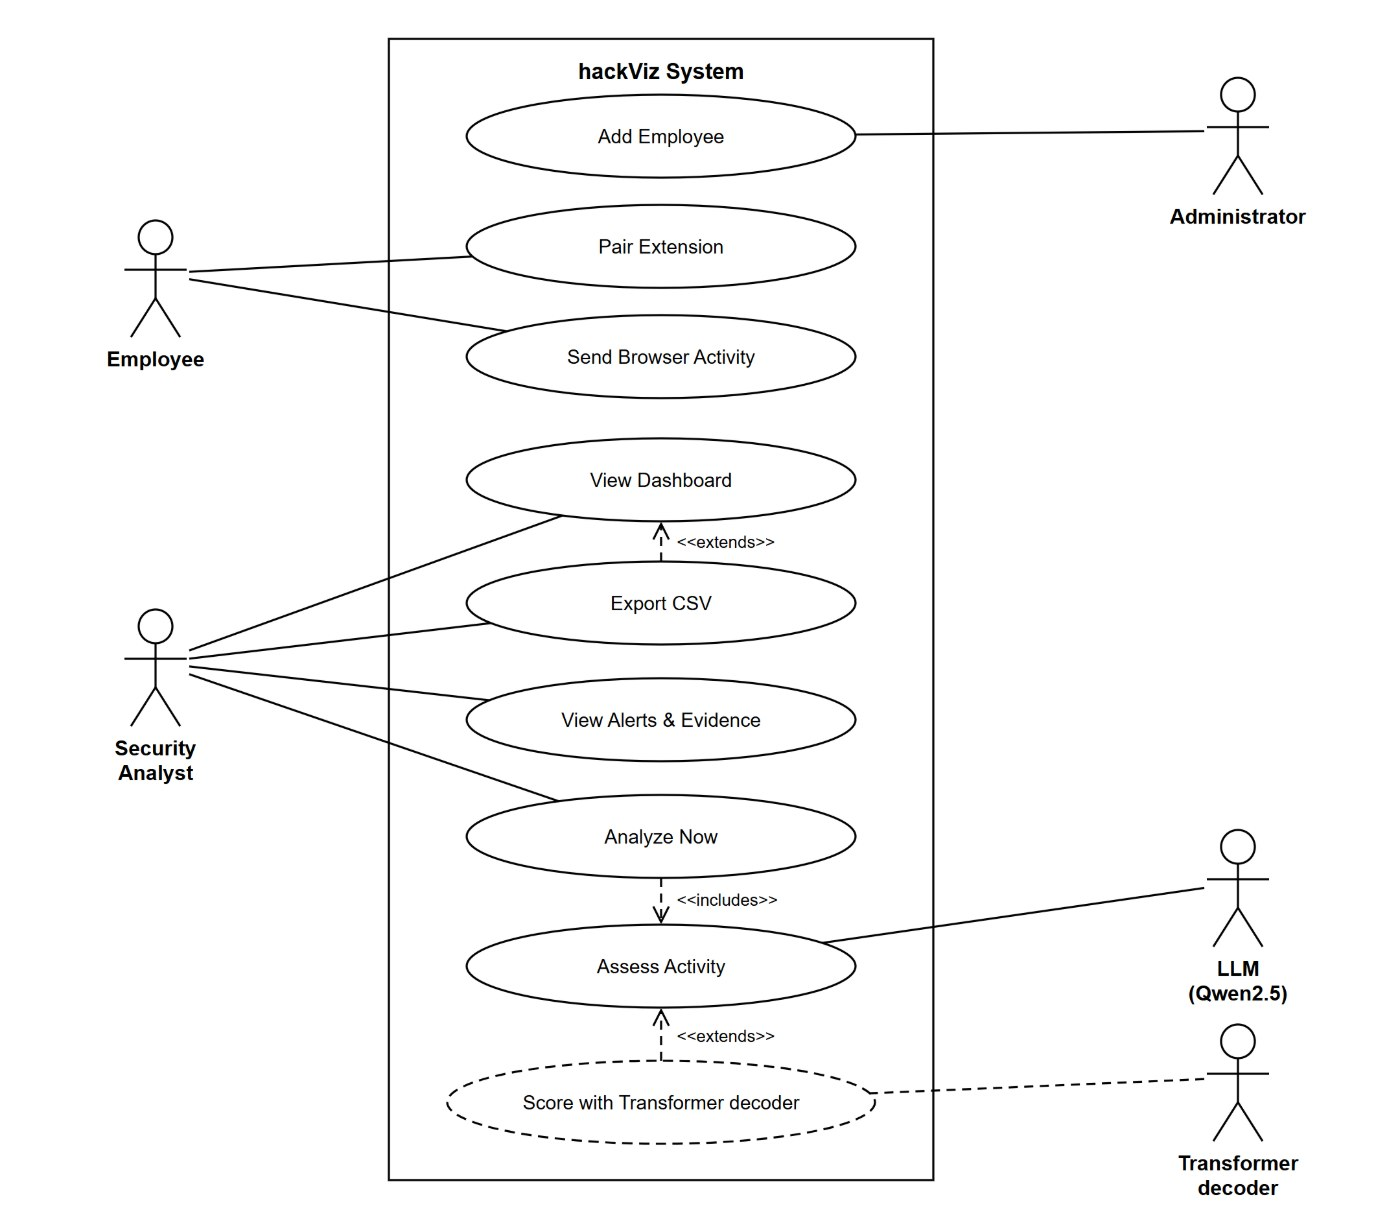
\includegraphics[width=\linewidth,height=0.68\textheight,keepaspectratio]{figures/uc_diagram.jpg}
\caption{Use case diagram of hackViz.}
\label{fig:uc}
\end{figure}

\subsection{Use Case Templates}

\uctable{UC-01}{Pair Chrome Extension}{Employee (primary)}
{Binds the Chrome extension to a verified employee after the employee agrees to monitoring.}
{Extension installed; employee exists in the directory.}
{1.~(AA) Employee opens the extension popup.\newline
2.~(SR) System shows the monitoring notice and the pairing form.\newline
3.~(AA) Employee ticks the consent box and enters the employee ID.\newline
4.~(SR) System verifies the ID and creates a session token.\newline
5.~(SR) System shows the employee's name and role; monitoring starts.}
{3a.~Consent not given: the pair button stays blocked.}
{4a.~Unknown ID: ``does not exist'' is shown.\newline 4b.~Backend unreachable: a connection error is shown.}
{Pairing is stored and browser events are collected.}

\uctable{UC-02}{Analyze Now}{Security Analyst (primary); LLM (secondary)}
{Runs an on-demand assessment of an employee's recent activity.}
{Employee has activity; the model is installed.}
{1.~(AA) Analyst opens an employee profile and clicks \emph{Analyze Now}.\newline
2.~(SR) System queues an analysis job and shows progress.\newline
3.~(SA) System performs \emph{Assess Activity} (UC-03).\newline
4.~(SR) System shows the new alert with its reason and evidence.}
{2a.~A job for this employee is already running: that job is shown.\newline
3a.~No new activity since the last assessment: the existing assessment is shown.}
{1a.~Employee has no activity: request rejected.\newline 3b.~Model times out: nothing saved, retried later.}
{A new assessment is stored, or the existing one is shown.}

\uctable{UC-03}{Assess Activity}{LLM (secondary); Transformer decoder (secondary, planned)}
{Assesses a window of an employee's events with the Transformer model.}
{Five new live events or 90 seconds of inactivity, or a request from UC-02.}
{1.~(SA) Select up to 35 new and 15 preceding events.\newline
2.~(SA) Summarise the baseline and compute indicators.\newline
3.~(SA) Send the prompt and JSON schema to the model.\newline
4.~(SR) Model returns an assessment.\newline
5.~(SA) Validate it and verify every evidence ID.\newline
6.~(SA) Save the assessment and move the cursor in one transaction.}
{5a.~Invalid response: one corrective retry.}
{4a.~Timeout or model missing: nothing saved, retried after a back-off.}
{Assessment stored; analysed events are never skipped.}

\uctable{UC-04}{View Alerts and Evidence}{Security Analyst (primary)}
{Lets the analyst review alerts and check the records they cite.}
{At least one assessment exists.}
{1.~(AA) Analyst opens the Anomaly Alerts page.\newline
2.~(SR) System lists alerts with risk, confidence and reason.\newline
3.~(AA) Analyst expands an alert and clicks an evidence ID.\newline
4.~(SR) System shows the original activity record.}
{1a.~Analyst filters alerts by risk level or employee.}
{4a.~Record not found: an error message is shown.}
{Analyst has checked the evidence behind the alert.}

\section{Activity Diagram and Swimlane Diagrams}

The activity diagram (Figure~\ref{fig:activity}) follows one browser event to a displayed alert. Decisions
carry guards in square brackets; flows that come back (waiting for more events, retrying an invalid model
response) re-enter through merge diamonds, and a fork/join shows that the alert and the analysis cursor are
saved together before the alert is shown. The LLM performs the assessment; the dashed action before it
is the planned Transformer decoder score. The swimlane diagram (Figure~\ref{fig:swim}) places each
action in the column of the participant that performs it.

\begin{figure}[H]
\centering
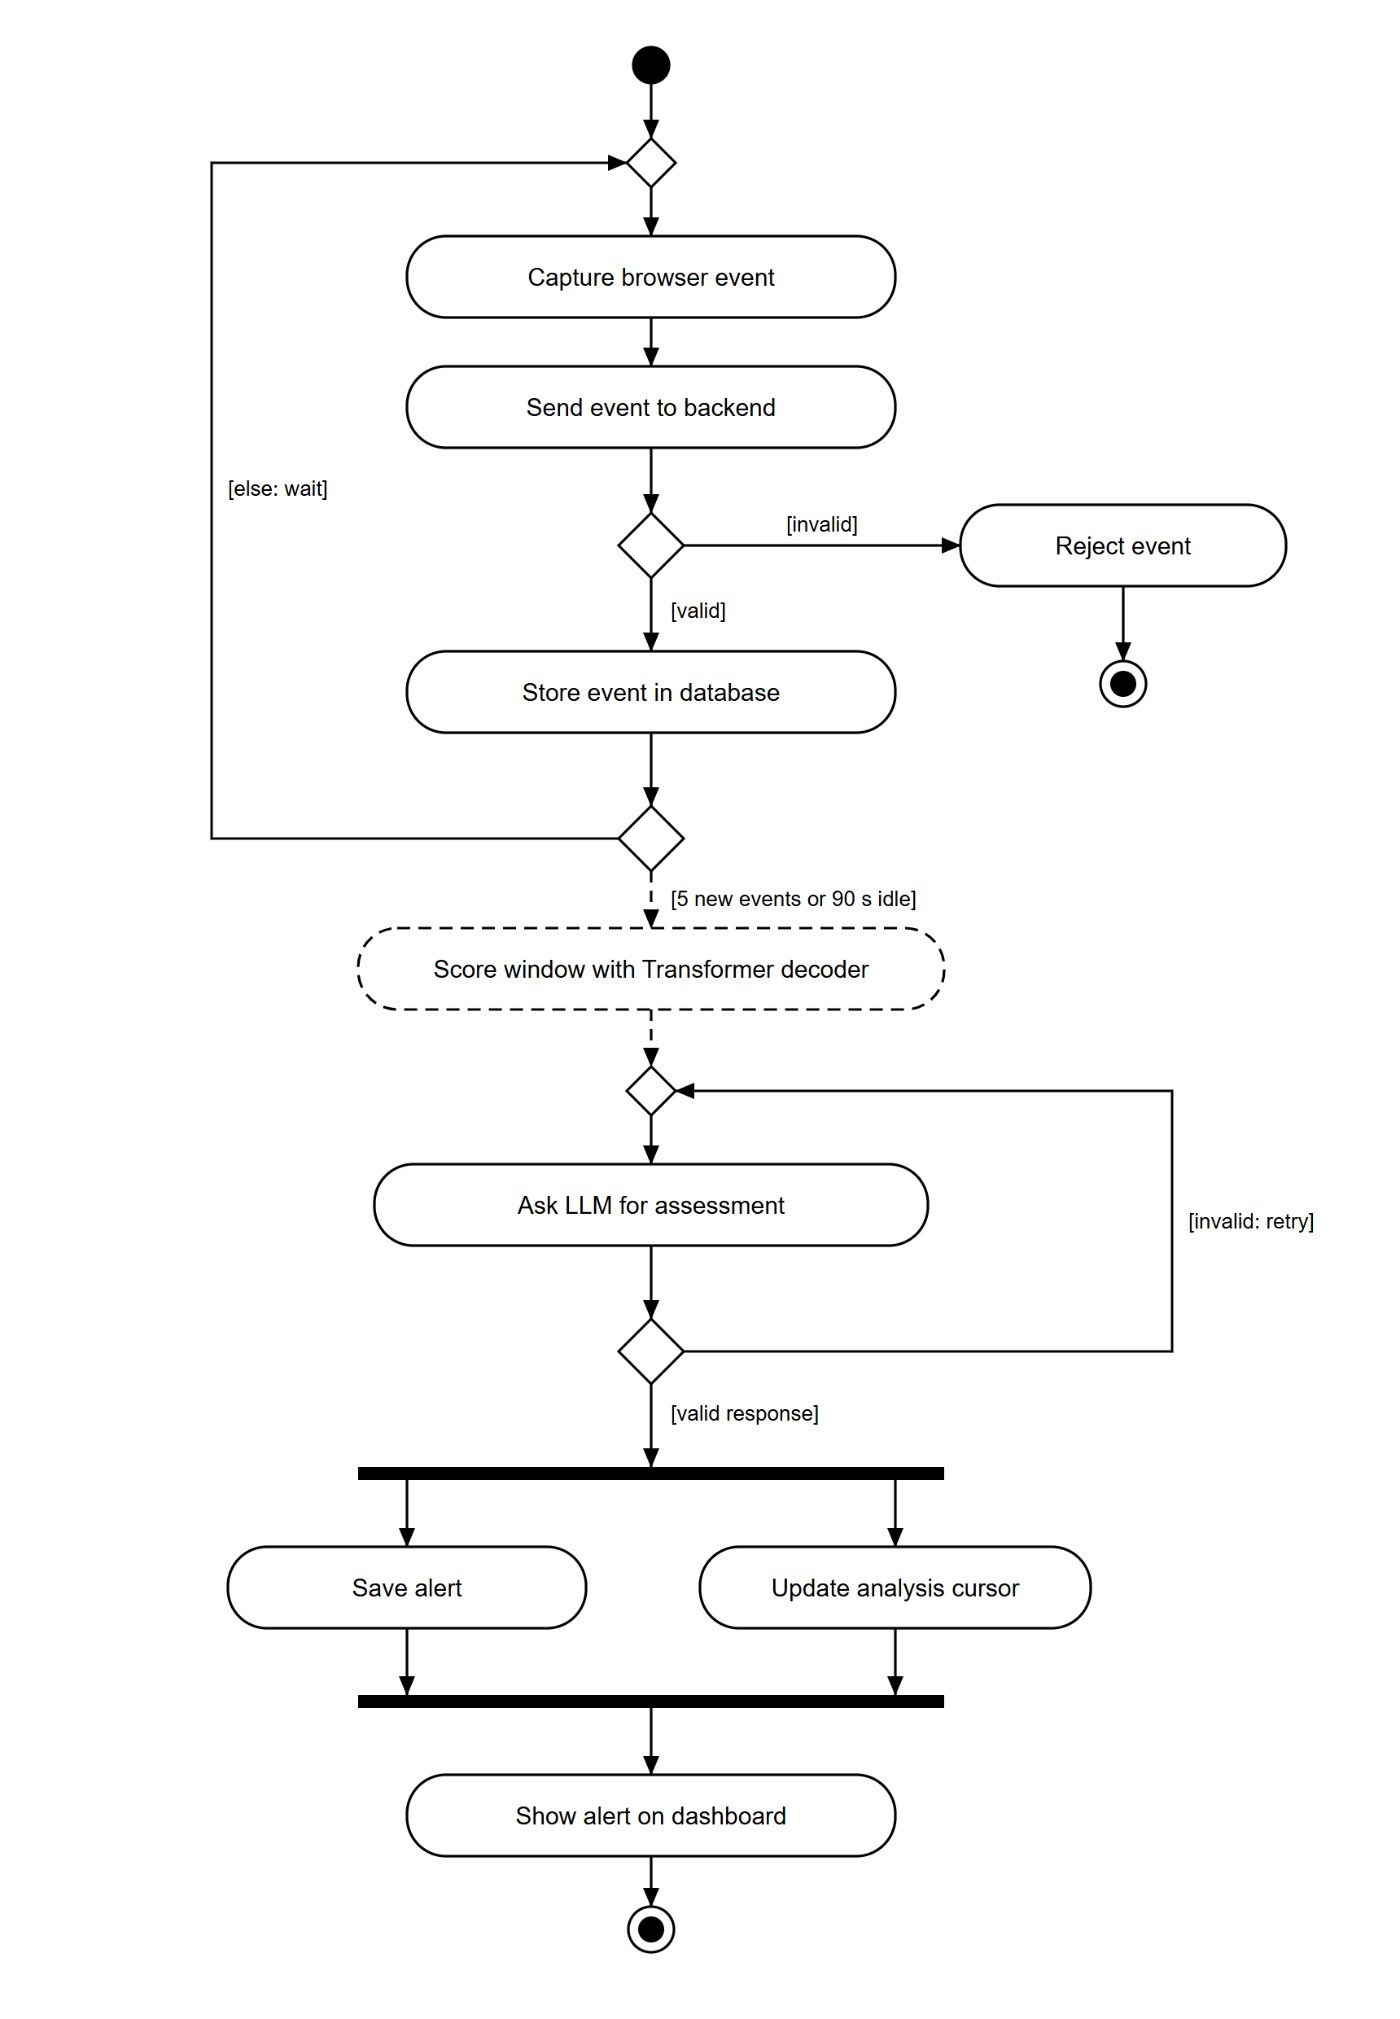
\includegraphics[width=\linewidth,height=0.7\textheight,keepaspectratio]{figures/activity_diagram.jpg}
\caption{Activity diagram: from browser event to displayed alert.}
\label{fig:activity}
\end{figure}

\begin{figure}[H]
\centering
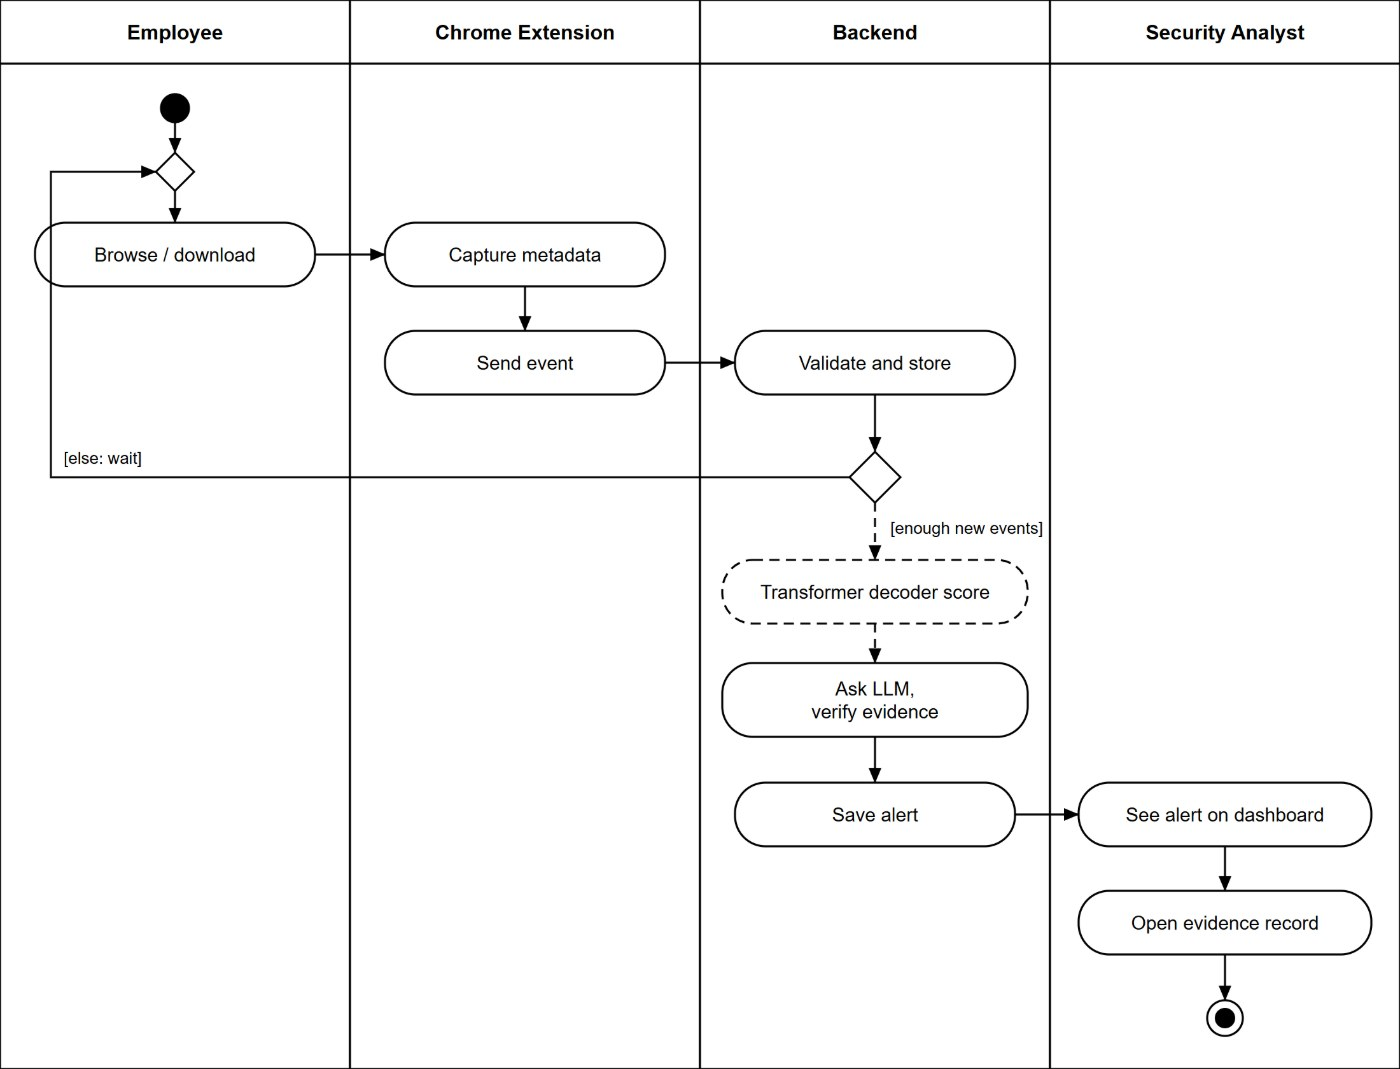
\includegraphics[width=\linewidth,height=0.7\textheight,keepaspectratio]{figures/swimlane_diagram.jpg}
\caption{Swimlane diagram.}
\label{fig:swim}
\end{figure}

\section{Data Flow Diagrams (DFDs)}

\subsection{DFD Level 0}

The context diagram (Figure~\ref{fig:dfd0}) shows hackViz as a single process (0) with its four external
entities (sources/sinks) and the major data flows: three inputs (browser activity, employee details,
Analyze Now request) and outputs to the analyst and to the LLM.

\begin{figure}[H]
\centering
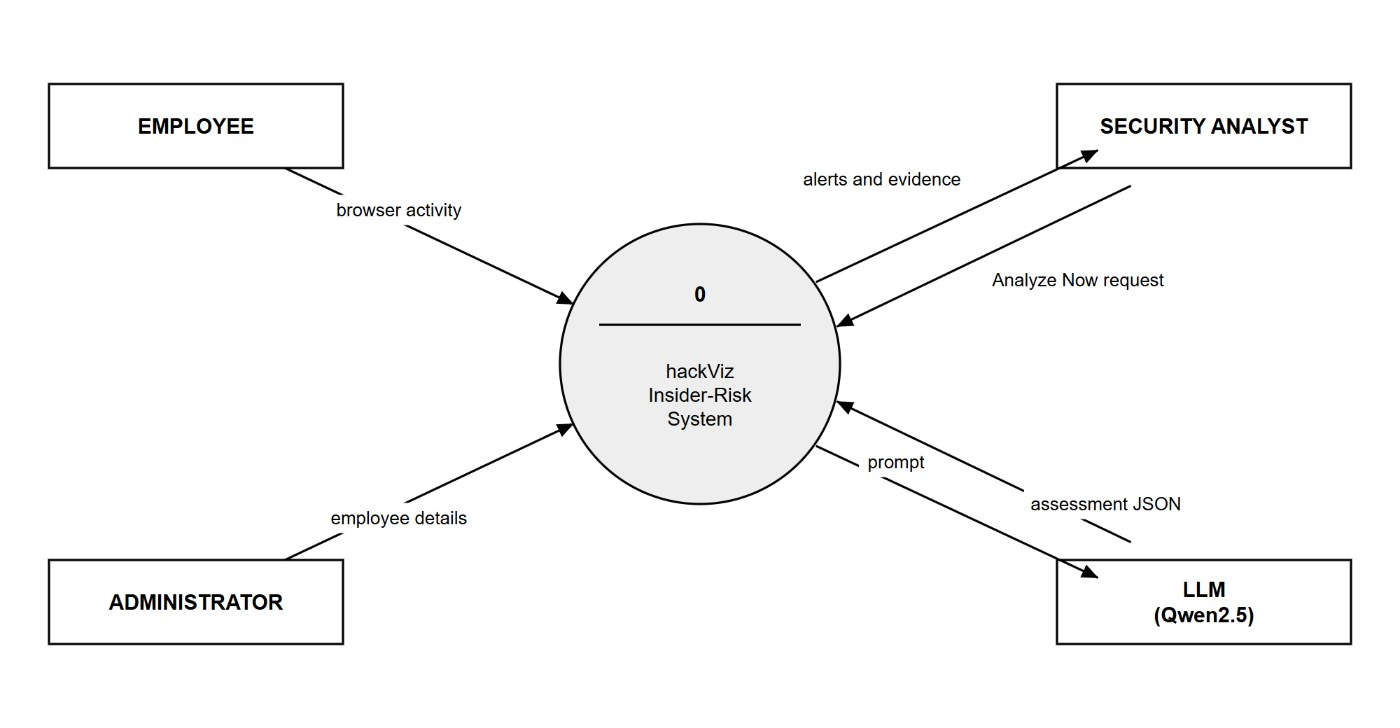
\includegraphics[width=0.92\linewidth]{figures/dfd_level0.jpg}
\caption{DFD level 0 (context diagram).}
\label{fig:dfd0}
\end{figure}

\subsection{DFD Level 1}

Level 1 (Figure~\ref{fig:dfd1}) decomposes the system into five processes and three data stores. It is
\textbf{balanced} with the context diagram: the same inputs and outputs appear and no new external flow is
added. Data reaches stores only through processes, and the Security Analyst is drawn twice to avoid
crossing lines. Process 4.0 sends the prompt to the LLM. The dashed process 6.0 is the planned
Transformer decoder: it would read the event sequence from D2 and pass an anomaly score to 4.0. It is an
internal process, so the balance with the context diagram is kept.

\begin{figure}[H]
\centering
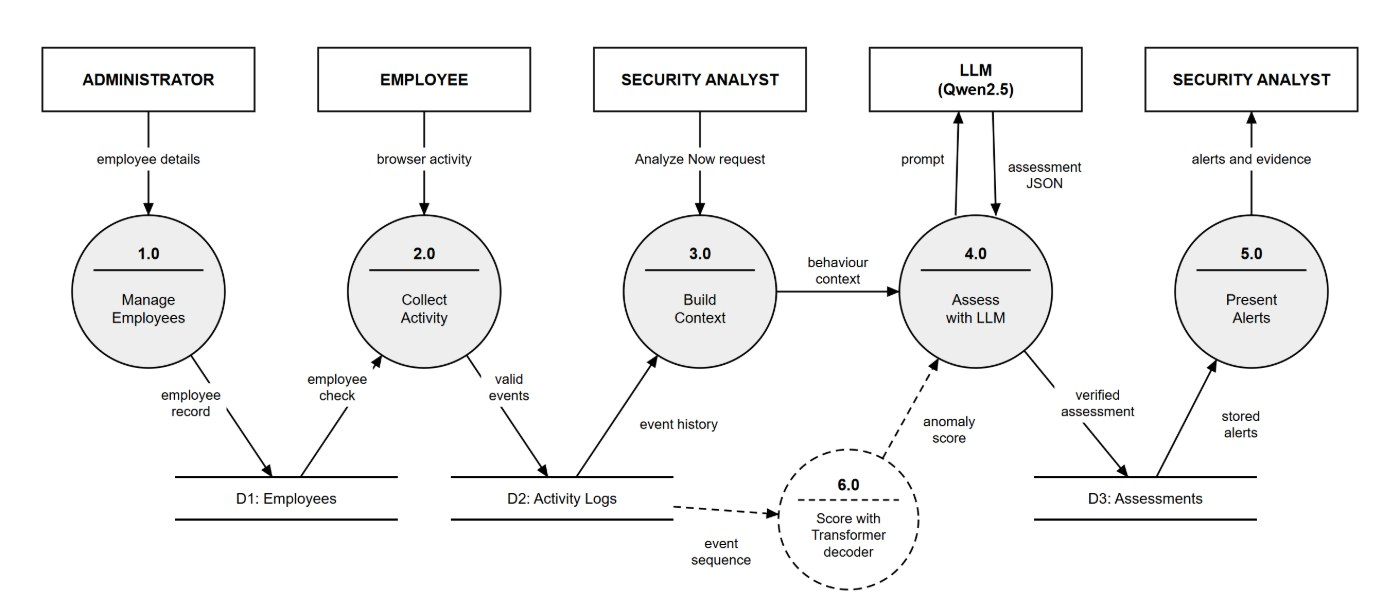
\includegraphics[width=\linewidth,height=0.62\textheight,keepaspectratio]{figures/dfd_level1.jpg}
\caption{DFD level 1 (balanced with level 0).}
\label{fig:dfd1}
\end{figure}

\subsection{DFD Level 2}

Level 2 (Figure~\ref{fig:dfd2}) decomposes process 4.0 (Assess with LLM) into 4.1--4.4. It keeps the
inputs (behaviour context, assessment JSON) and outputs (prompt, verified assessment) of 4.0, so it is
balanced with Level 1.

\begin{figure}[H]
\centering
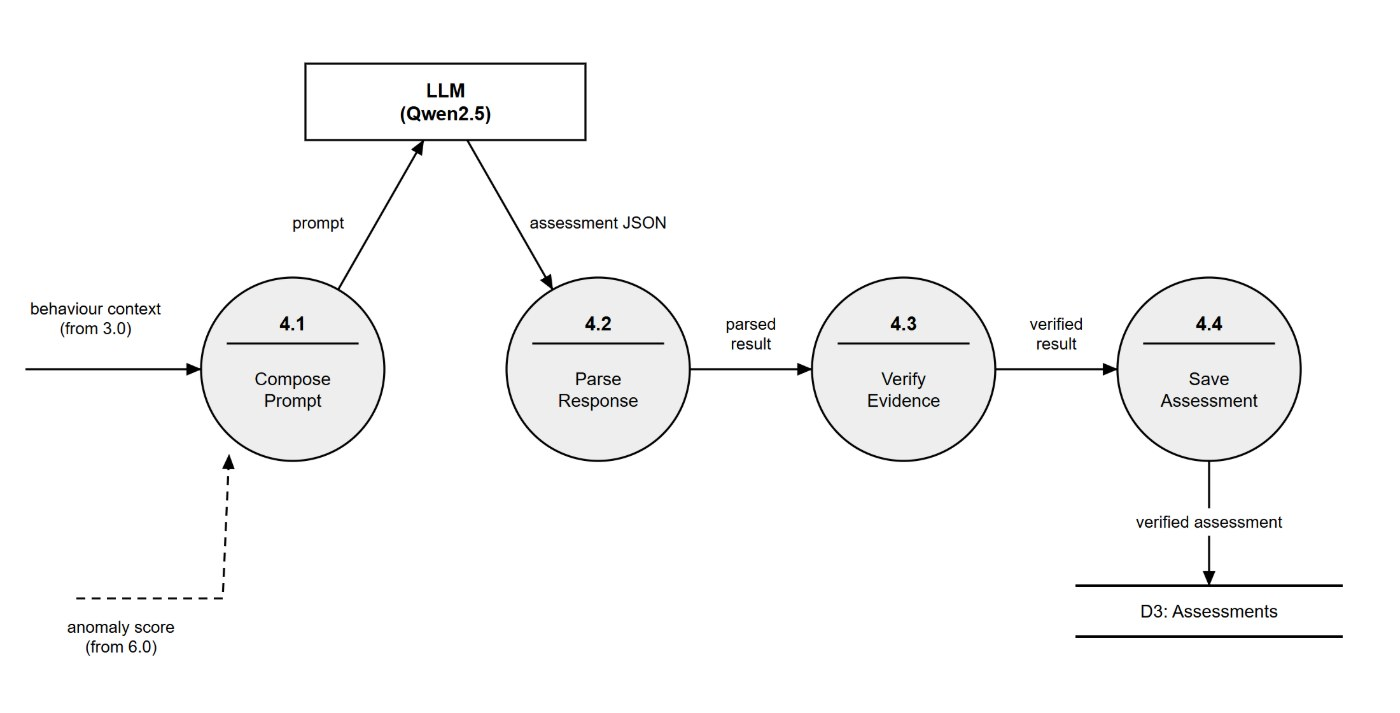
\includegraphics[width=0.9\linewidth,height=0.55\textheight,keepaspectratio]{figures/dfd_level2.jpg}
\caption{DFD level 2: decomposition of process 4.0.}
\label{fig:dfd2}
\end{figure}

\section{Software Requirement Specification in IEEE Format}

This section follows the structure of IEEE Std 830~\cite{ieee830}.

\subsection{Purpose, Scope and Definitions}

\paragraph{Purpose.} To specify the functional and non-functional requirements of hackViz and record how
far each is met.

\paragraph{Scope.} As defined in Section~\ref{sec:scope}; the system assists analysts and takes no
enforcement action.

\paragraph{Definitions.} \emph{Assessment}: the system's judgement of a window of activity (risk level,
confidence, reason, evidence, action). \emph{Analysis window}: new live events of one employee plus
preceding context. \emph{Evidence ID}: database ID of a cited activity record. \emph{LLM}: large
language model, here Qwen2.5-3B-Instruct. \emph{Pairing}: binding the extension to a verified employee
after consent.

\subsection{Overall Description}

\paragraph{Product perspective.} A self-contained system made of the parts described in
Section~\ref{sec:arch}, communicating over HTTP and SQL on one machine.

\paragraph{Product functions.} Employee management; extension pairing; collection, validation and
storage of activity; baselines and indicators; automatic and on-demand assessment with evidence
verification; alert review; CSV export; system monitoring.

\begin{table}[H]
\centering
\small
\caption{User classes.}
\label{tab:users}
\begin{tabularx}{\linewidth}{@{}lYl@{}}
\toprule
\textbf{User class} & \textbf{Responsibilities} & \textbf{Skill} \\
\midrule
Security Analyst & Reviews dashboards, alerts and evidence; triggers analysis; exports data & Medium \\
System Administrator & Adds employees, seeds or resets the dataset, monitors health & High \\
Monitored Employee & Pairs the extension after consent and browses normally & Low \\
\bottomrule
\end{tabularx}
\end{table}

\paragraph{Operating environment.} Windows 10/11, 16\,GB RAM, no GPU; Python 3.12; Node.js 20+;
PostgreSQL 16; Ollama with \texttt{qwen2.5:3b}; Google Chrome (Manifest V3).

\paragraph{Constraints.} PostgreSQL only; the model must run locally; no paid or cloud AI services; no
model training; ingestion must not wait for inference; only metadata may be collected.

\paragraph{Assumptions.} Records carry timestamps and employee IDs; only authorised staff use the
dashboard; employees are informed before pairing.

\subsection{Specific Requirements}

\begin{table}[H]
\centering
\small
\caption{Functional requirements and status.}
\label{tab:fr}
\begin{tabularx}{\linewidth}{@{}lYl@{}}
\toprule
\textbf{ID} & \textbf{Requirement} & \textbf{Status} \\
\midrule
FR-01 & Authenticate users and enforce role-based access & Not implemented \\
FR-02 & Ingest historical records and live browser activity & Implemented \\
FR-03 & Validate and normalise all events into one schema & Implemented \\
FR-04 & Order events per employee and build analysis windows & Implemented \\
FR-05 & Assess each window with a risk level and confidence & Implemented \\
FR-06 & Explain each assessment with a reason and verified evidence & Implemented \\
FR-07 & Rank and filter employees and alerts by risk & Partial (no date filter) \\
FR-08 & Pair the extension only with a verified, consenting employee & Implemented \\
FR-09 & Collect navigation/download metadata without query strings & Implemented \\
FR-10 & Analyse automatically (5 events / 90\,s idle) and on demand & Implemented \\
FR-11 & Never re-run inference on an unchanged window & Implemented \\
FR-12 & Confirm or dismiss alerts and audit analyst actions & Not implemented \\
FR-13 & Export activity as CSV & Implemented \\
FR-14 & Report backend, database, model and extension status & Implemented \\
FR-15 & Train LSTM/GRU/Transformer autoencoders & Not implemented \\
\bottomrule
\end{tabularx}
\end{table}

\begin{table}[H]
\centering
\small
\caption{Non-functional requirements and status.}
\label{tab:nfr}
\begin{tabularx}{\linewidth}{@{}lYl@{}}
\toprule
\textbf{Category} & \textbf{Requirement} & \textbf{Status} \\
\midrule
Performance & One analysis on a CPU in under 3 minutes; ingestion never waits & Implemented \\
Reliability & Invalid records never corrupt data; no event skipped after failures & Implemented \\
Security & Input validation, token-bound pairing, local-only model; login and audit missing & Partial \\
Privacy & Metadata only, with consent, stored locally & Implemented \\
Usability & Analysts find suspicious activity and understand explanations & Implemented \\
Maintainability & Separate route, schema, model and service modules & Implemented \\
Explainability & Every alert cites verified records; evidence is a lead, not proof & Implemented \\
\bottomrule
\end{tabularx}
\end{table}

\paragraph{Data requirements.} Every event has an ID, employee ID, timestamp, type, domain, URL
without query or fragment, optional file name and source. Page content, form data, e-mail bodies,
keystrokes and credentials are never collected. The dataset contains no labels.

\section{User Stories and Story Cards}

Each user story is written on a story card with its priority, story points, acceptance criteria and
current status.

\vspace{6pt}
\noindent
\storycard{US-01}{As a \textbf{Security Analyst}, I want a ranked list of suspicious activity so that I
can prioritise triage.}{High}{3}{ranked by risk; filterable by entity and date; refreshes when new
assessments arrive.}{Partial (no date filter)}\hfill
\storycard{US-02}{As a \textbf{Security Analyst}, I want to see why an alert was raised so that I can
judge whether it is a real risk.}{High}{5}{reason shown with the analysed events; evidence highlighted;
labelled as a lead, not proof.}{Implemented}

\vspace{8pt}
\noindent
\storycard{US-03}{As a \textbf{Security Analyst}, I want to open the original record behind any
evidence ID so that I can verify the claim.}{High}{2}{every evidence ID is clickable and shows the
stored record.}{Implemented}\hfill
\storycard{US-04}{As a \textbf{Monitored Employee}, I want to know what is collected and to stop it so
that my privacy is respected.}{High}{3}{notice and consent before pairing; Disconnect stops collection
immediately.}{Implemented}

\vspace{8pt}
\noindent
\storycard{US-05}{As a \textbf{Security Analyst}, I want suspicious activity flagged without automatic
blocking so that a human decides.}{High}{2}{no automatic action; high-risk activity surfaced for
review.}{Implemented}\hfill
\storycard{US-06}{As a \textbf{System Administrator}, I want to add employees from the dashboard so that
new staff can be monitored without a restart.}{Medium}{2}{form with validation; duplicate IDs rejected;
employee usable immediately.}{Implemented}

\vspace{8pt}
\noindent
\storycard{US-07}{As a \textbf{Security Analyst}, I want to confirm or dismiss an alert so that my
decision is recorded.}{High}{2}{confirm/dismiss on every alert; decision timestamped and
attributed.}{Not implemented}\hfill
\storycard{US-08}{As an \textbf{ML Engineer}, I want to compare LSTM, GRU and Transformer autoencoders
so that the best detector is chosen.}{Medium}{5}{same held-out split; F1, false-positive rate and latency
reported.}{Not implemented}

% ===================================================== 3. DESIGN PHASE
\chapter{Design Phase}

This chapter gives two significant cases of the class and sequence diagrams. The design applies the main design
concepts: \emph{modularity} (separate modules for routes, schemas, models, analysis and the model client),
\emph{information hiding} (each model is reached only through the AnomalyModel interface), \emph{functional
independence} (each module has one task and few connections) and \emph{abstraction} (data classes describe
records; the worker hides how an analysis is queued and retried).

\section{Class Diagram}

Figure~\ref{fig:classdomain} shows the persistent classes stored in PostgreSQL. Each record cannot exist
without its employee, so these are \emph{compositions} with multiplicity 1 at the Employee end; an Anomaly
\emph{cites} one or more ActivityLog records (association). Figure~\ref{fig:classanalysis} shows the
analysis classes: the worker is composed of its jobs and runs the Analyzer, which \emph{uses} an abstract
AnomalyModel and \emph{creates} an LLMAssessment (dependency). LLM (implemented, Qwen2.5 with 36 decoder
layers) and TransformerDecoder (dashed, planned) are \emph{generalisations} of AnomalyModel, so the
Transformer decoder can be added later without changing the Analyzer.

\begin{figure}[H]
\centering
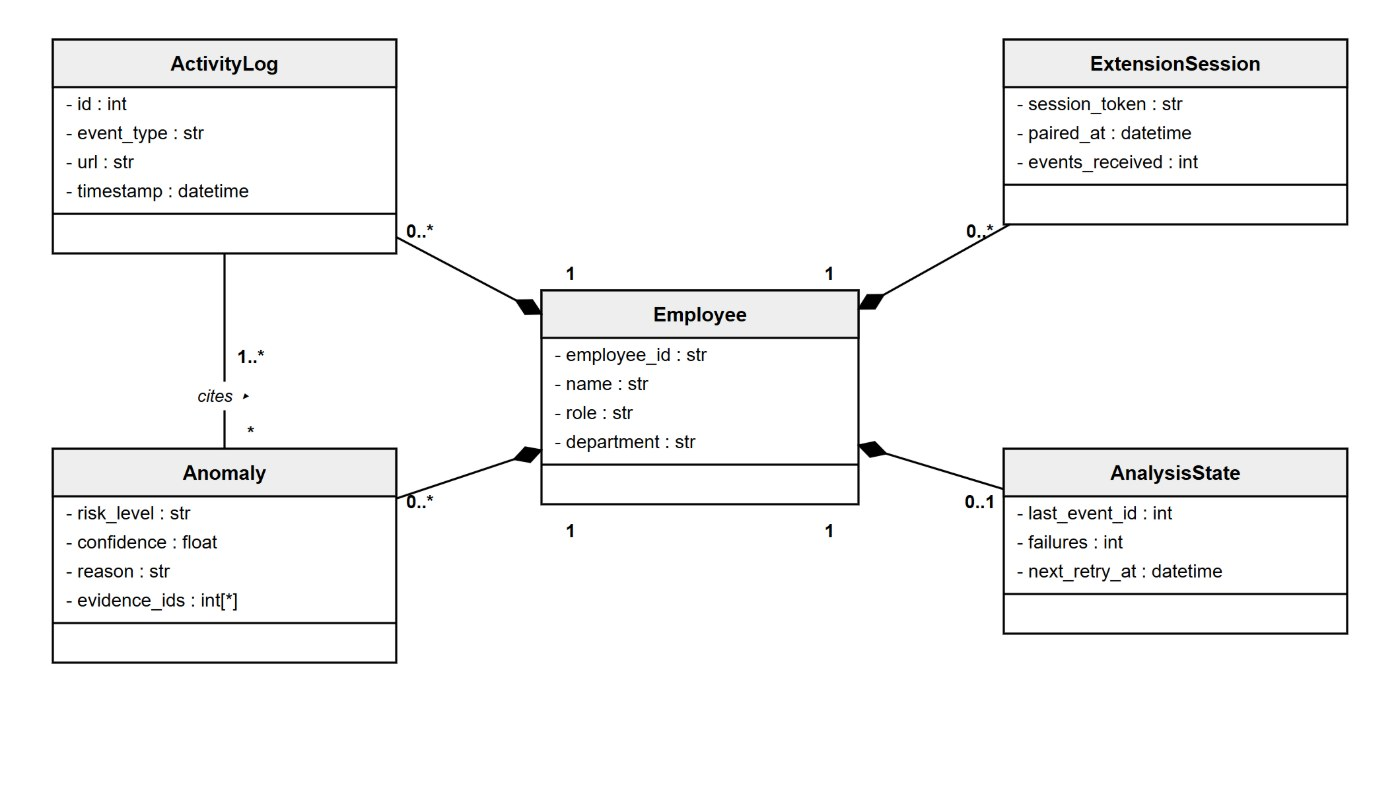
\includegraphics[width=\linewidth]{figures/class_domain.jpg}
\caption{Class diagram 1: domain (persistence) classes.}
\label{fig:classdomain}
\end{figure}

\begin{figure}[H]
\centering
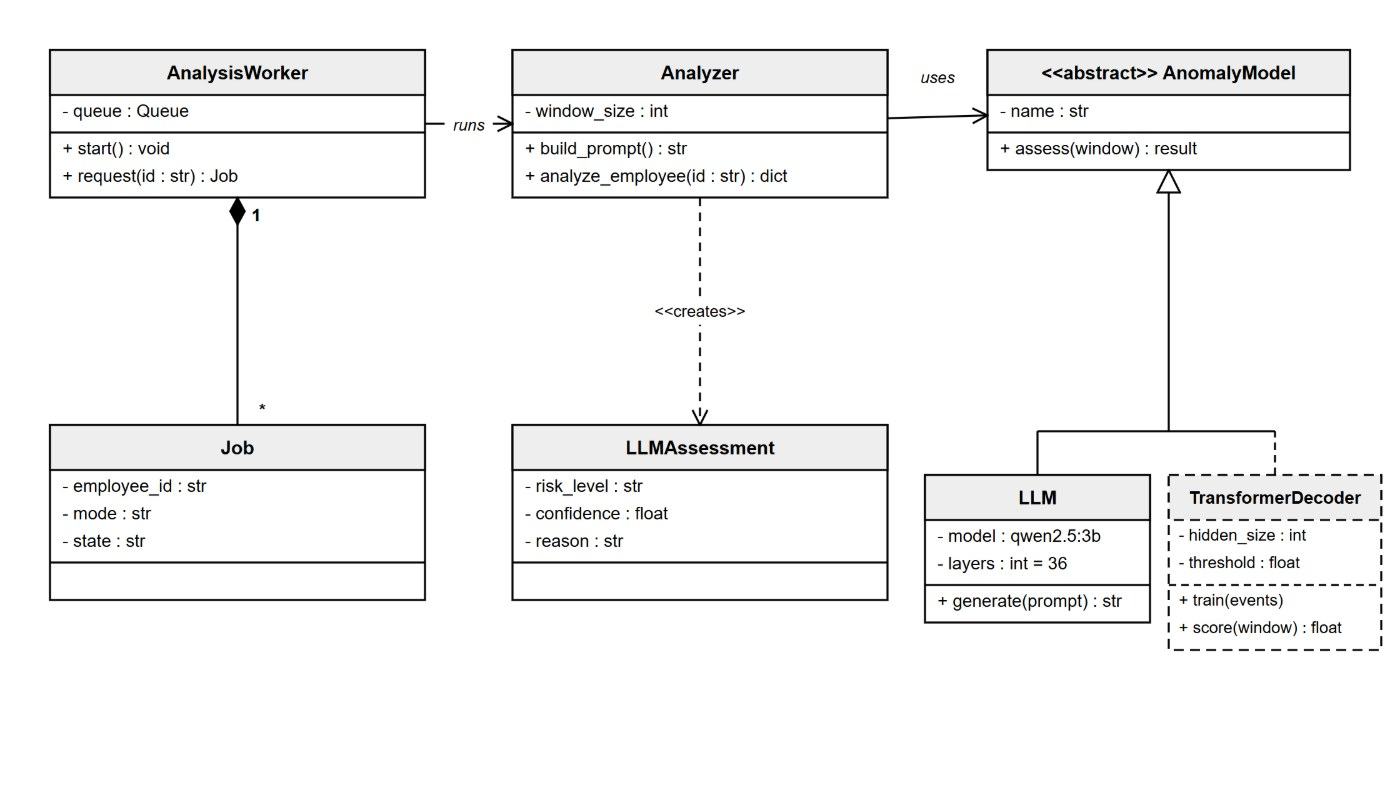
\includegraphics[width=\linewidth]{figures/class_analysis.jpg}
\caption{Class diagram 2: analysis and model-access classes.}
\label{fig:classanalysis}
\end{figure}

\section{Sequence Diagram}

Figure~\ref{fig:seq1} shows pairing the extension and sending an event; Figure~\ref{fig:seq2} shows the
on-demand \emph{Analyze Now} case, in which the Backend sends the prompt to the LLM; the dashed lifeline
is the planned Transformer decoder. Solid arrows are requests and dashed arrows are replies.

\begin{figure}[H]
\centering
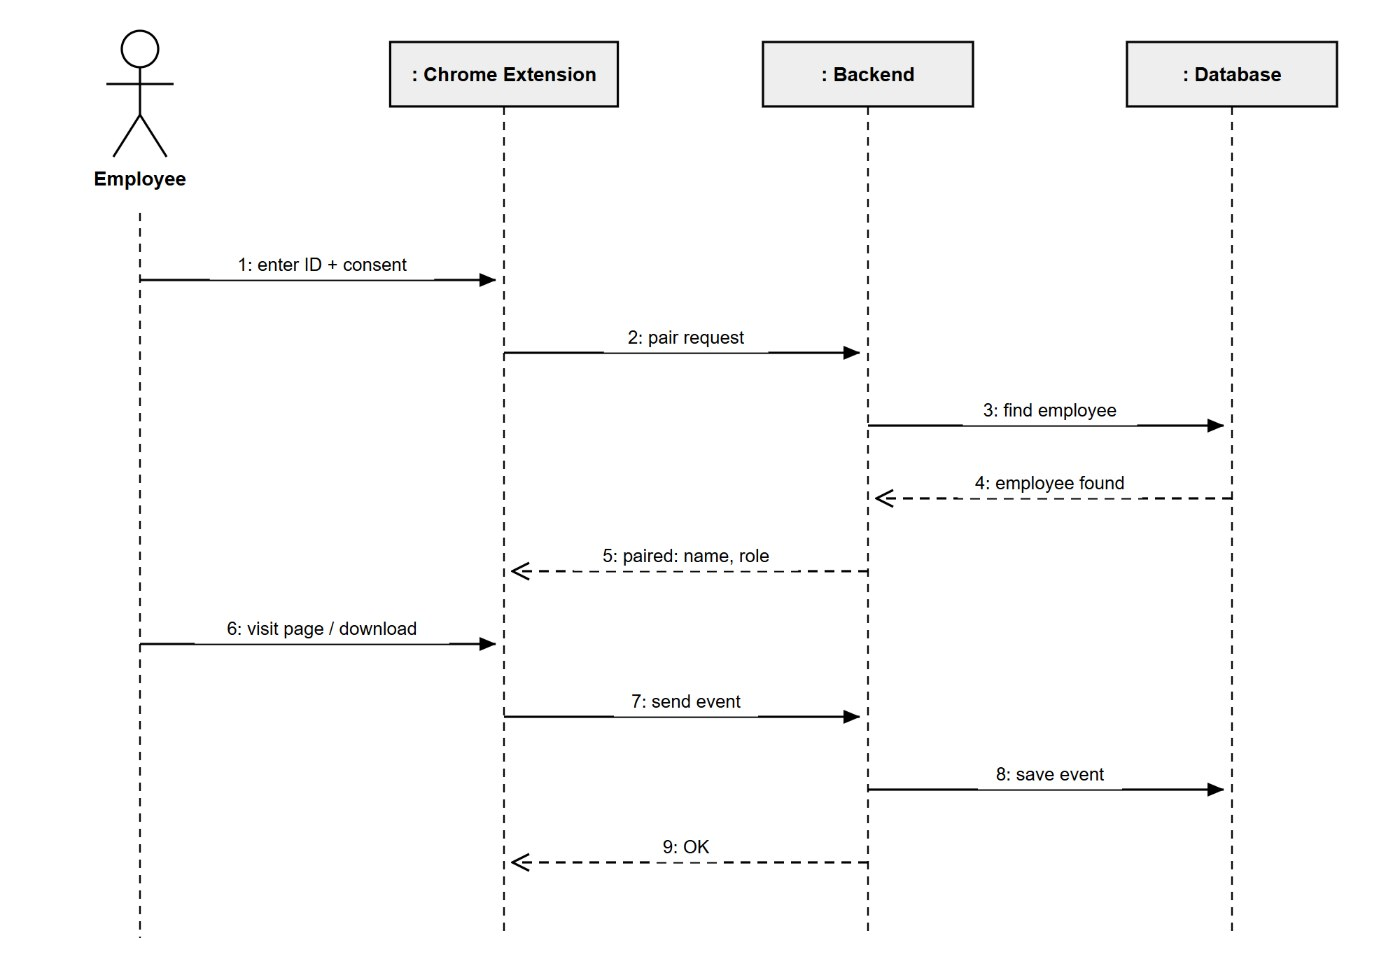
\includegraphics[width=\linewidth,height=0.72\textheight,keepaspectratio]{figures/sequence_diagram.jpg}
\caption{Sequence diagram 1: pairing and sending activity.}
\label{fig:seq1}
\end{figure}

\begin{figure}[H]
\centering
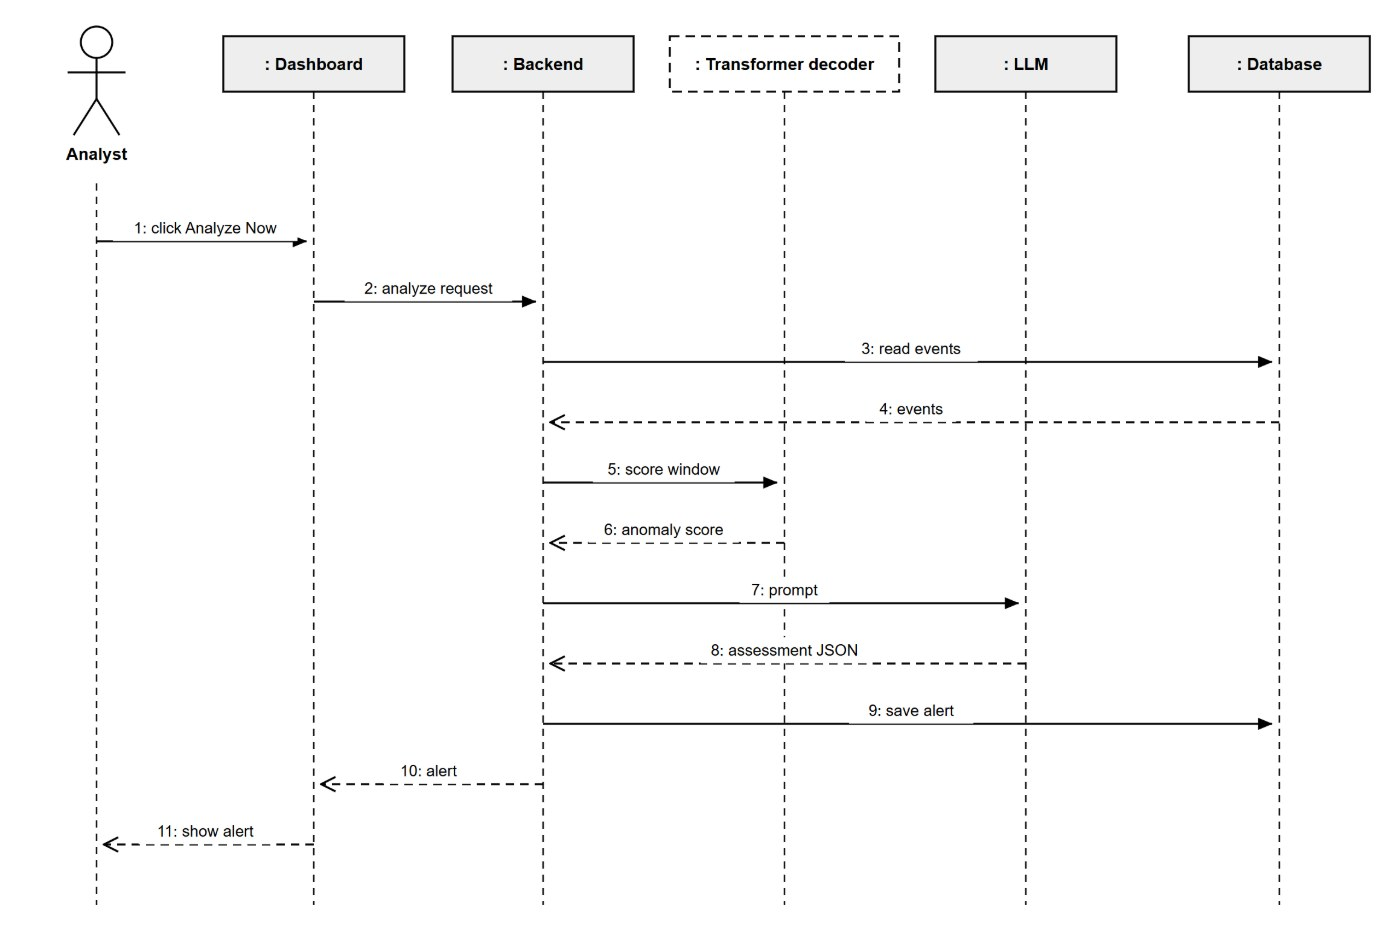
\includegraphics[width=\linewidth,height=0.62\textheight,keepaspectratio]{figures/sequence_analyze.jpg}
\caption{Sequence diagram 2: on-demand analysis (Analyze Now).}
\label{fig:seq2}
\end{figure}

% ===================================================== 4. IMPLEMENTATION
\chapter{Implementation}

The backend is written in Python 3.12 with FastAPI, SQLAlchemy 2 and psycopg 3 on PostgreSQL 16; the
dashboard in React 18 with Vite; the extension in JavaScript for Chrome Manifest V3. The model is
\texttt{qwen2.5:3b} served by Ollama on the CPU with temperature 0.1 and a JSON schema.

\section{Screenshots}

\begin{figure}[H]
\centering
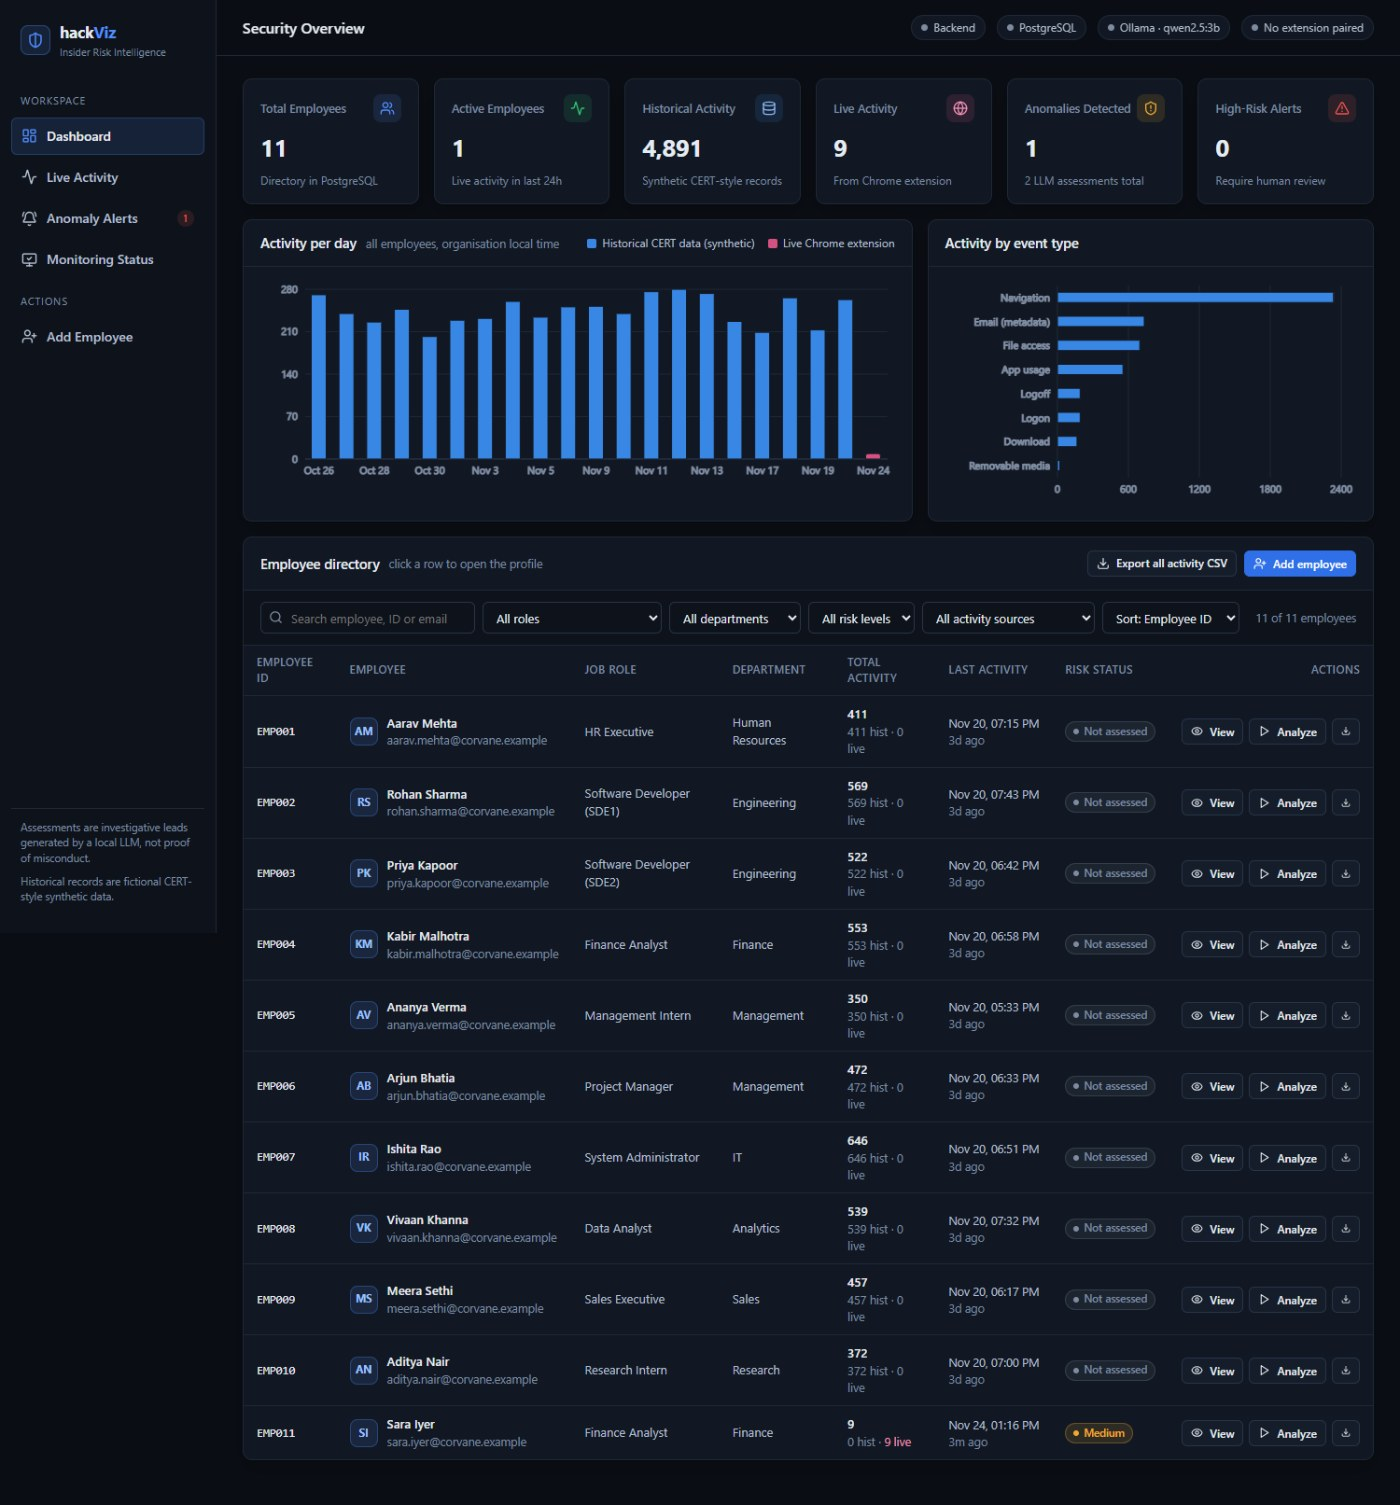
\includegraphics[width=\linewidth,height=0.4\textheight,keepaspectratio]{figures/ui_dashboard.jpg}
\caption{Dashboard: summary cards, activity charts and employee directory.}
\end{figure}

\begin{figure}[H]
\centering
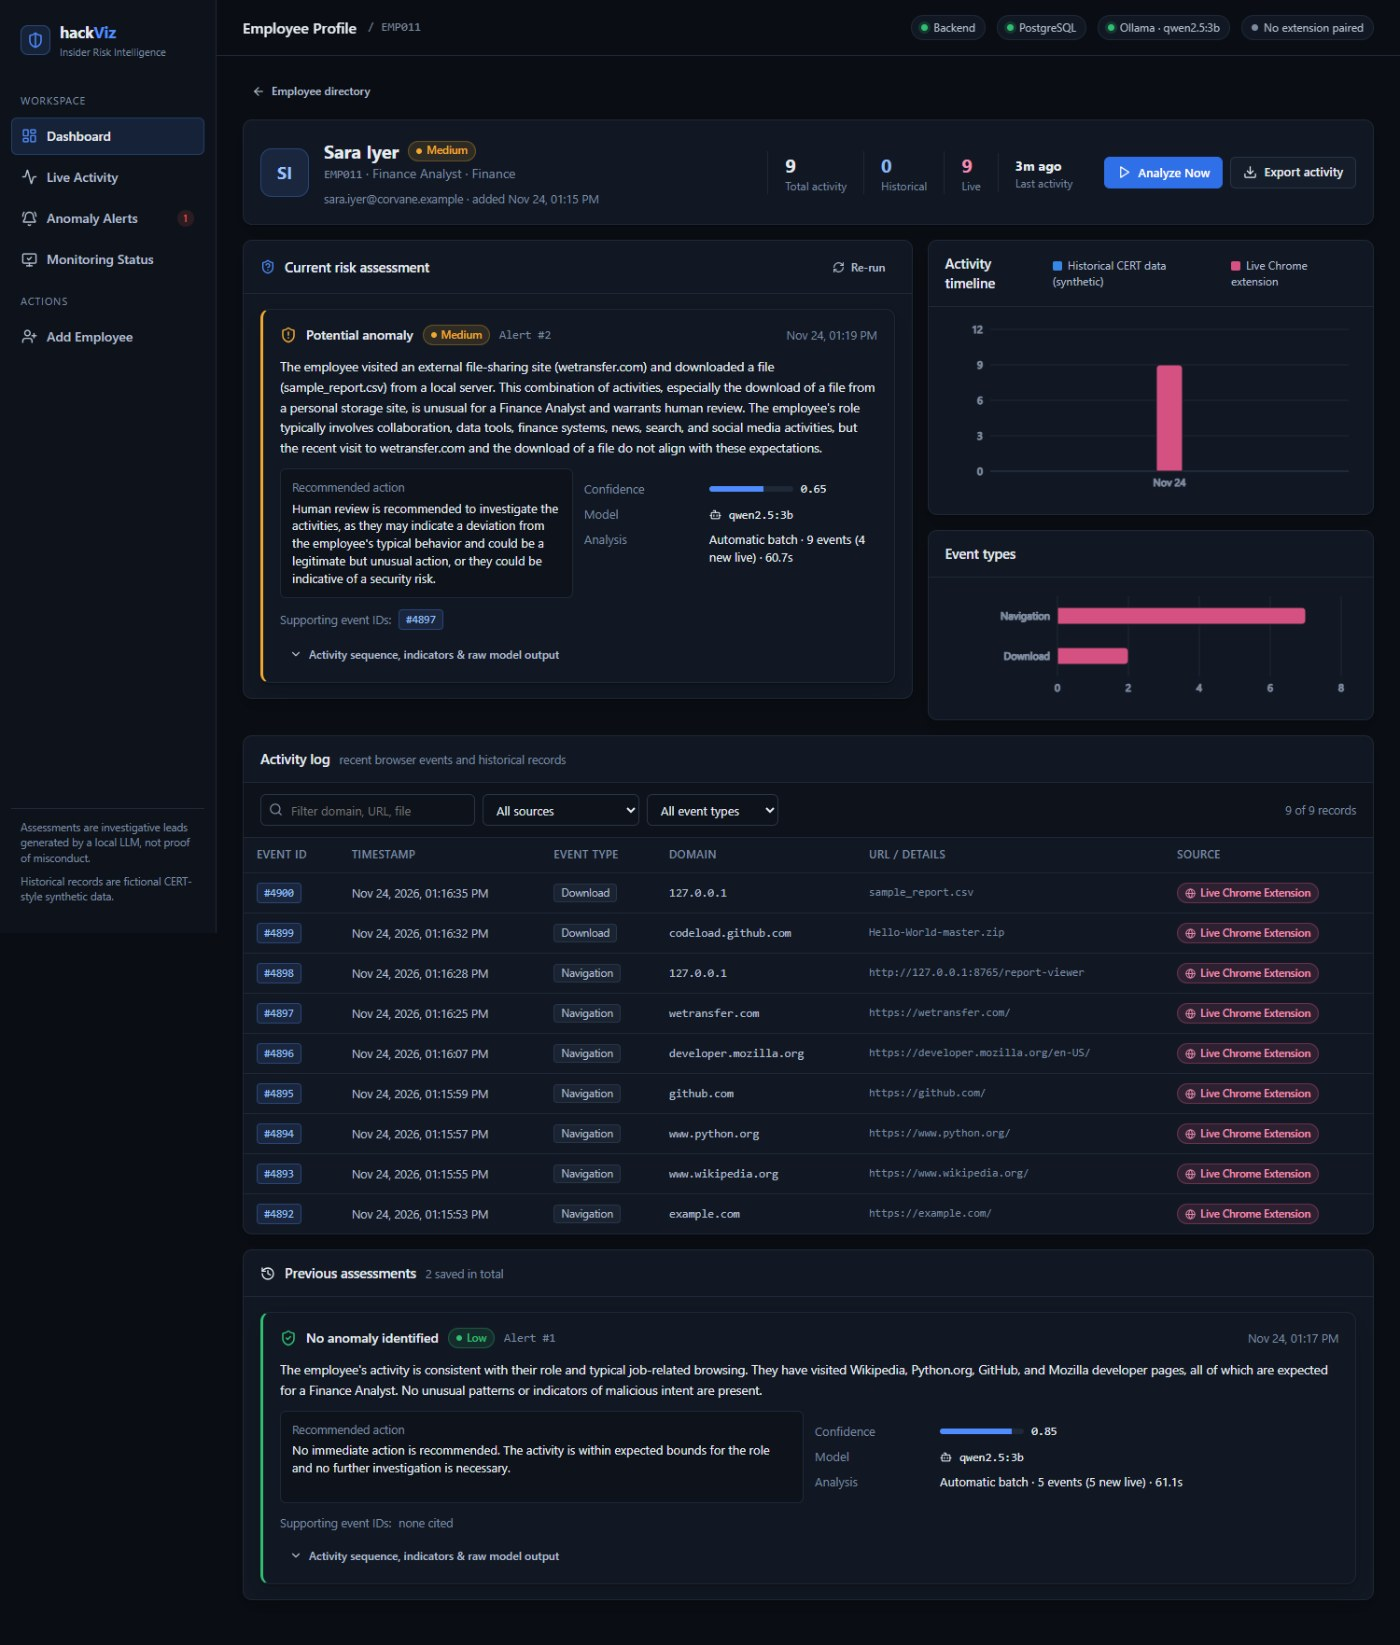
\includegraphics[width=\linewidth,height=0.4\textheight,keepaspectratio]{figures/ui_profile.jpg}
\caption{Employee profile with \emph{Analyze Now}, timeline and assessments.}
\end{figure}

\begin{figure}[H]
\centering
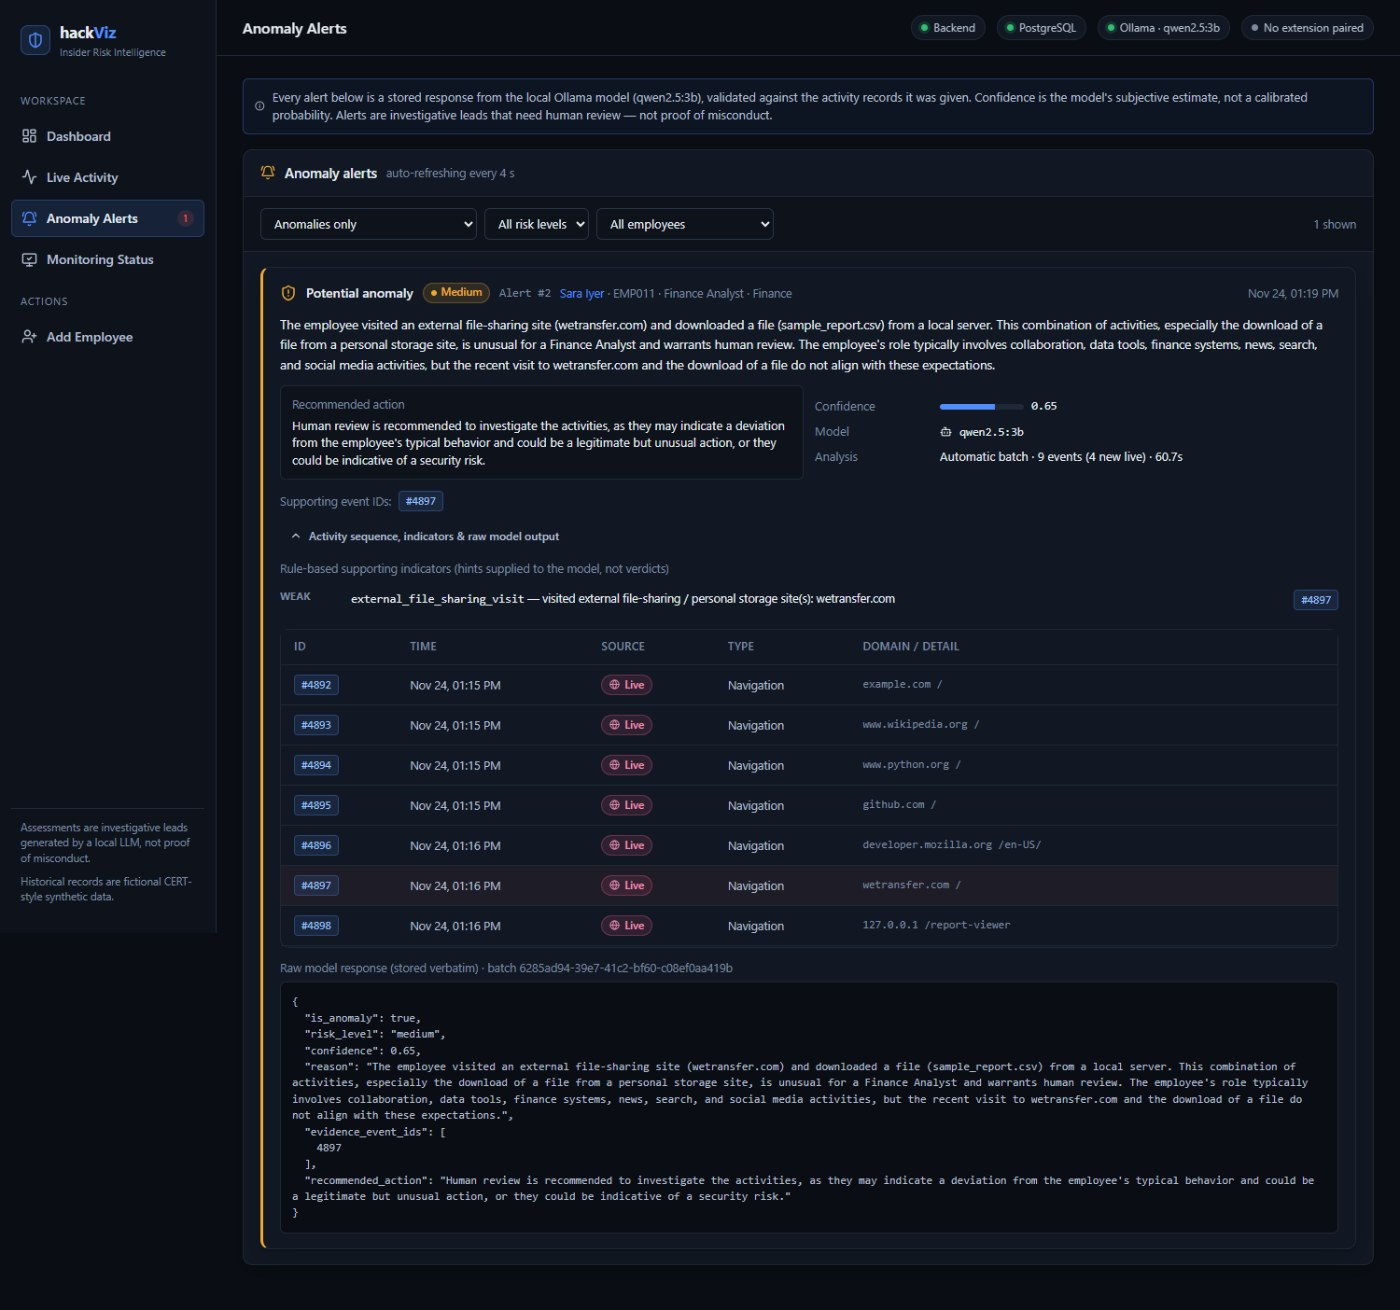
\includegraphics[width=\linewidth,height=0.4\textheight,keepaspectratio]{figures/ui_alert_expanded.jpg}
\caption{An alert with its explanation, evidence, indicators and raw model output.}
\end{figure}

\begin{figure}[H]
\centering
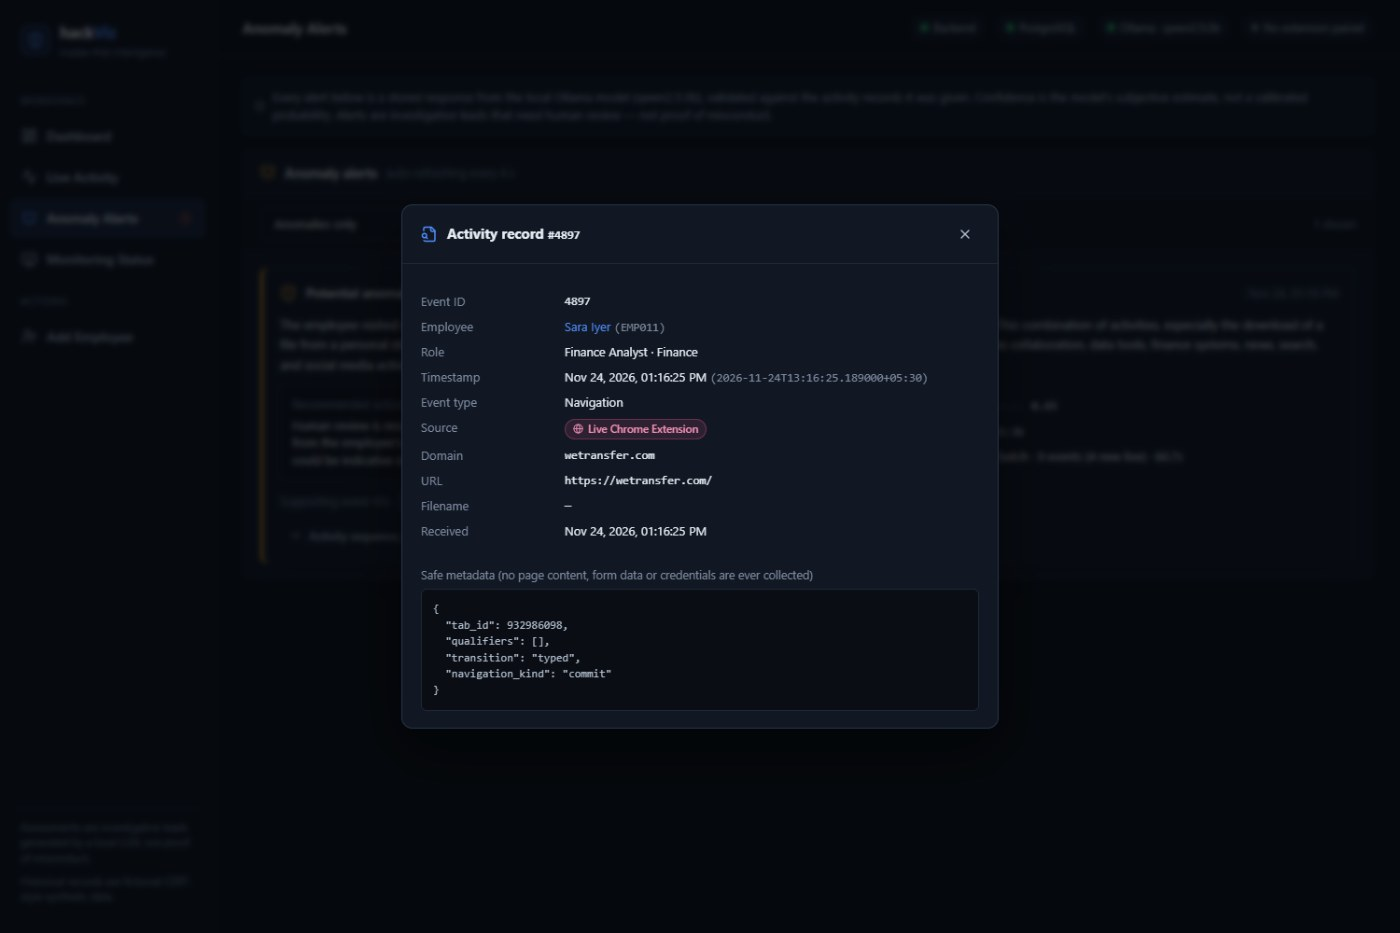
\includegraphics[width=0.9\linewidth,height=0.38\textheight,keepaspectratio]{figures/ui_evidence_modal.jpg}
\caption{The original activity record opened from an evidence ID.}
\end{figure}

\begin{figure}[H]
\centering
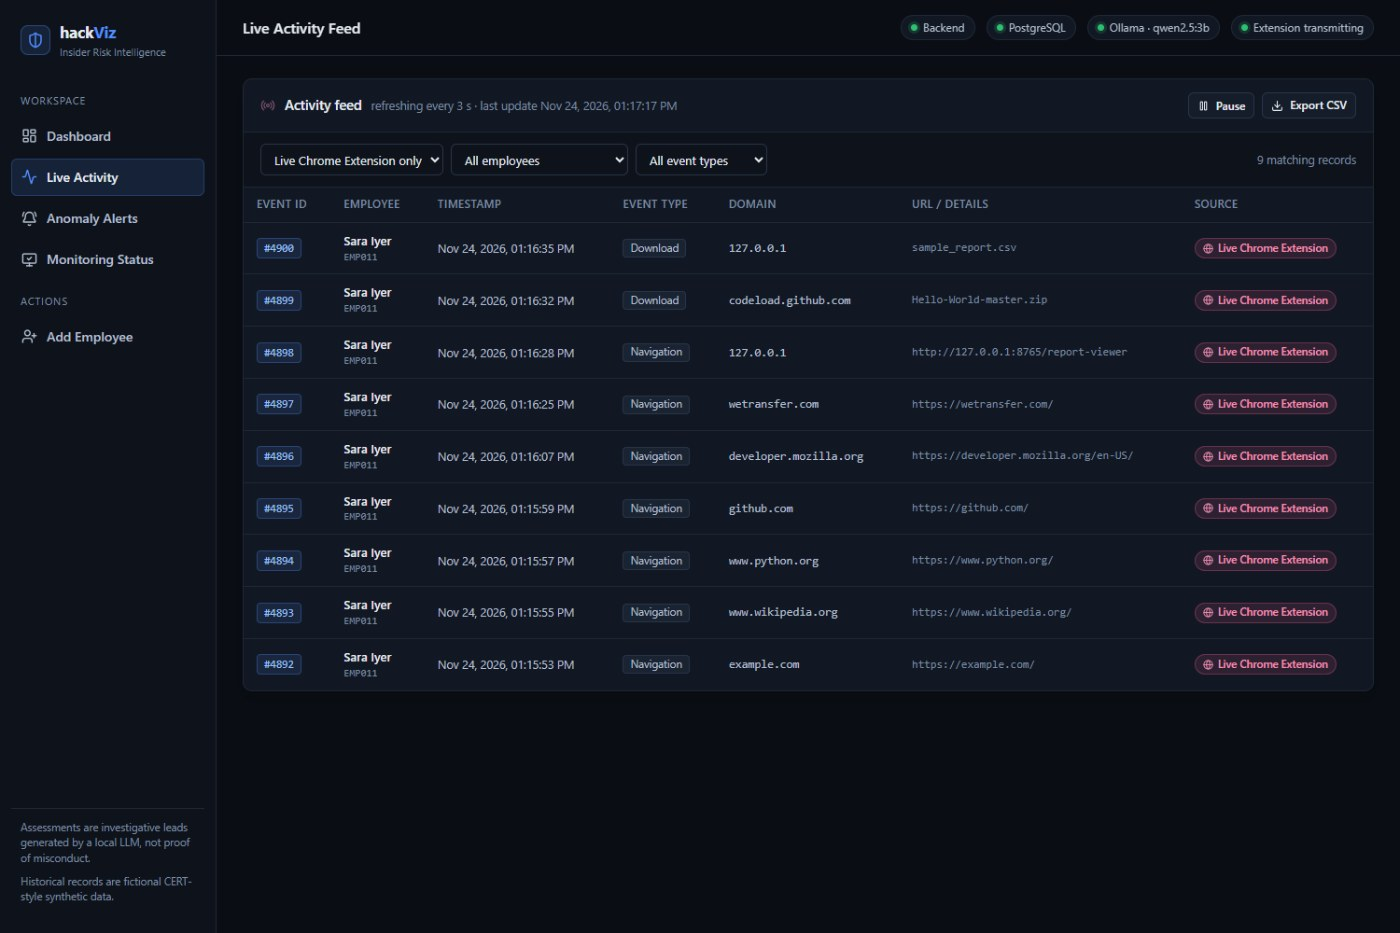
\includegraphics[width=\linewidth,height=0.4\textheight,keepaspectratio]{figures/05_live_feed.jpg}
\caption{Live activity feed showing events from the extension.}
\end{figure}

\begin{figure}[H]
\centering
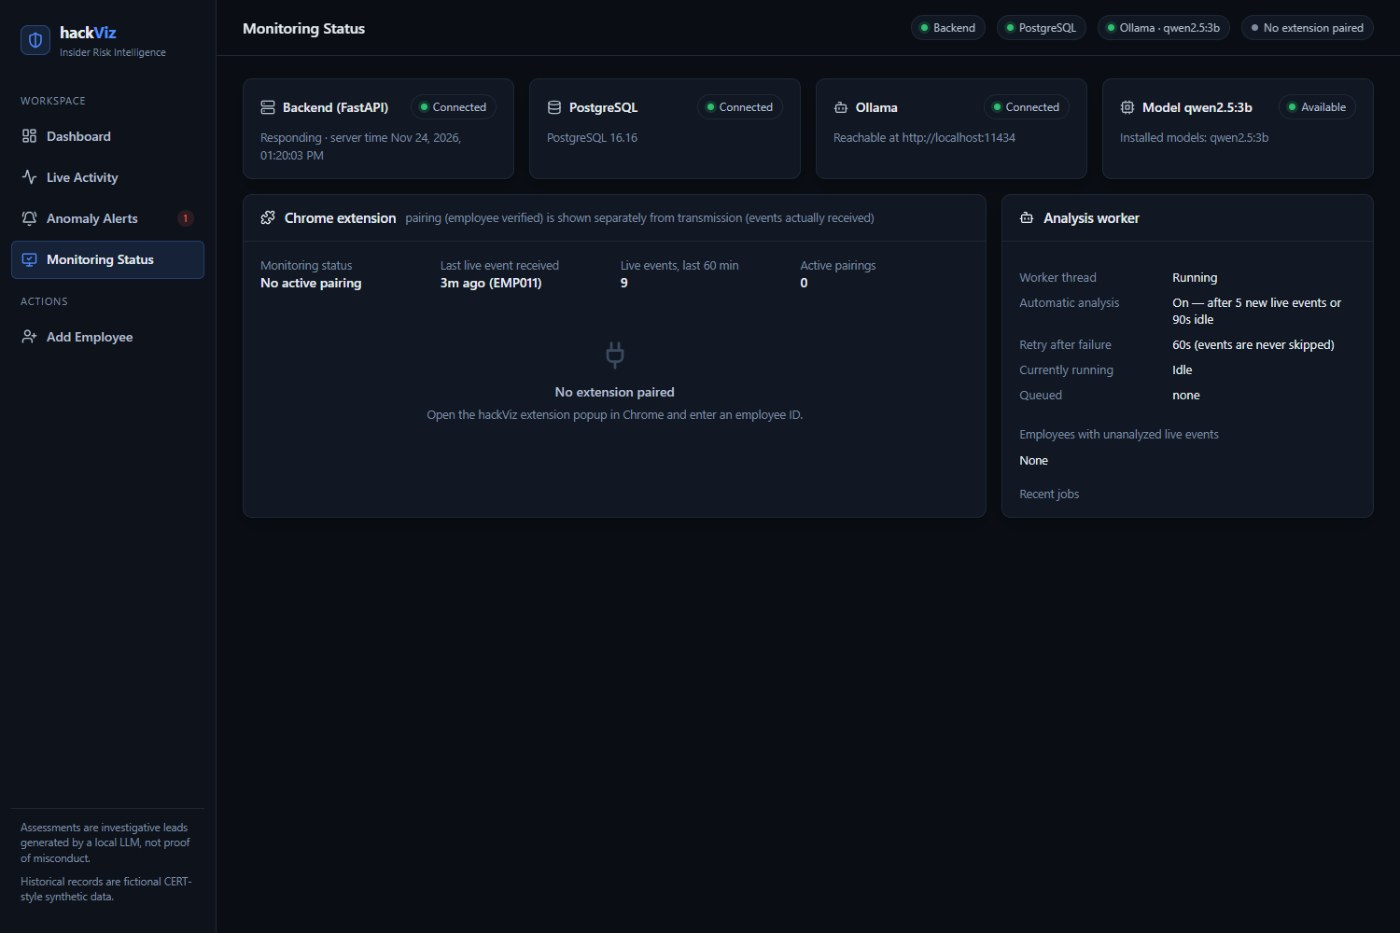
\includegraphics[width=\linewidth,height=0.4\textheight,keepaspectratio]{figures/ui_monitoring.jpg}
\caption{Monitoring status: backend, database, model, pairings and worker.}
\end{figure}

\begin{figure}[H]
\centering
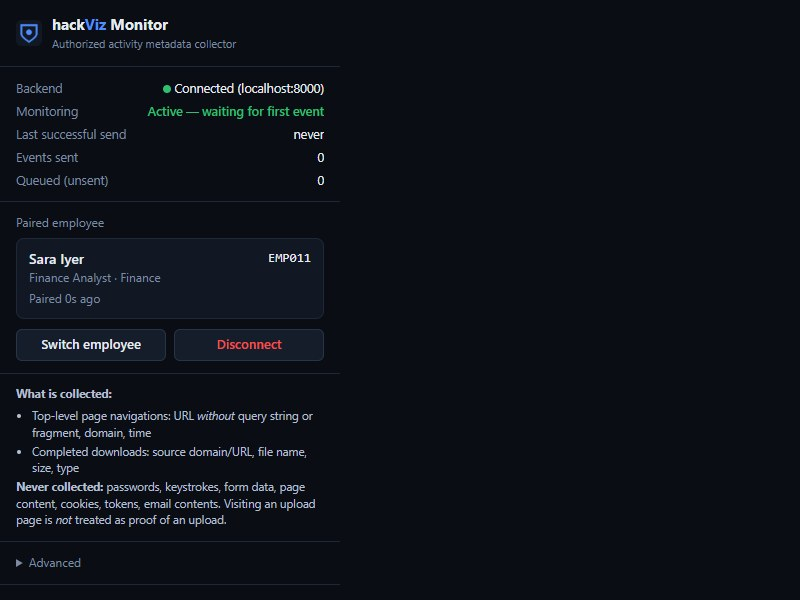
\includegraphics[width=0.42\linewidth]{figures/01_extension_paired.jpg}
\caption{Extension popup after pairing.}
\end{figure}

% ===================================================== 5. TESTING
\chapter{Testing}

\section{Test Plan}

\begin{table}[H]
\centering
\small
\caption{Test plan.}
\label{tab:testplan}
\begin{tabularx}{\linewidth}{@{}>{\bfseries}p{3.0cm}Y@{}}
\toprule
Objective & Show that every implemented requirement works with real components: real PostgreSQL, real
  model inference and a real browser. No model response is mocked. \\
Items tested & Response validation and evidence verification; indicators and prompt; REST API;
  database; dataset generator; model integration; Chrome extension; dashboard. \\
Levels & Unit (19 tests), integration with API and database (26), model integration (9),
  end-to-end with the installed Chrome (26 steps), dashboard checks (8). \\
Environment & Windows 11, 16\,GB RAM, CPU only; PostgreSQL 16.16; Ollama 0.40.16 with
  \texttt{qwen2.5:3b}; Chrome 158. Tests use a separate database recreated for every run. \\
Tools & pytest, FastAPI TestClient, Puppeteer with the installed Chrome. \\
Entry criteria & Services running; model installed; test database reachable. \\
Exit criteria & All automated tests and end-to-end steps pass; no console errors on the dashboard. \\
Not tested & Load with many users; accuracy on labelled data (the dataset has no labels). \\
\bottomrule
\end{tabularx}
\end{table}

\section{Test Cases}

Table~\ref{tab:tests} lists the automated test cases. TC-03 runs seven invalid inputs, so 48 test cases
give 54 executions; all passed.

{\small
\begin{xltabular}{\linewidth}{@{}lp{1.7cm}Yl@{}}
\caption{Automated test cases and results.}\label{tab:tests}\\
\toprule
\textbf{ID} & \textbf{Type} & \textbf{Test and expected behaviour} & \textbf{Result} \\
\midrule
\endfirsthead
\toprule
\textbf{ID} & \textbf{Type} & \textbf{Test and expected behaviour} & \textbf{Result} \\
\midrule
\endhead
\bottomrule
\endfoot
TC-01 & Unit & A valid model response is accepted & Pass \\
TC-02 & Unit & IDs like ``\#102'' and upper-case risk levels are normalised & Pass \\
TC-03 & Unit & Invalid risk, confidence out of range, inconsistent flags, empty reason, missing action
  are rejected (7 cases) & Pass \\
TC-04 & Unit & A response with a missing field is rejected & Pass \\
TC-05 & Unit & Invented evidence IDs are removed and noted & Pass \\
TC-06 & Unit & An anomaly citing only invented IDs is rejected & Pass \\
TC-07 & Unit & A no-anomaly result without evidence is accepted & Pass \\
TC-08 & Unit & JSON in a code fence is parsed; plain text is rejected & Pass \\
TC-09 & Unit & Sensitive download then wetransfer.com gives a strong indicator & Pass \\
TC-10 & Unit & One unfamiliar website gives no strong indicator & Pass \\
TC-11 & Unit & Admin portal expected for a system administrator, flagged for an intern & Pass \\
TC-12 & Unit & Download burst detected; off-hours browsing alone gives nothing & Pass \\
TC-13 & Unit & A 35-event prompt is labelled and stays compact & Pass \\
TC-14 & Integration & Health and status report database, model and monitoring & Pass \\
TC-15 & Integration & Directory lists the ten employees & Pass \\
TC-16 & Integration & Employee created; duplicate gives HTTP 409 & Pass \\
TC-17 & Integration & Invalid employee fields give HTTP 422 & Pass \\
TC-18 & Integration & Unknown employee gives HTTP 404 & Pass \\
TC-19 & Integration & Query string removed; duplicate client event not stored twice & Pass \\
TC-20 & Integration & Download path stored as file name only & Pass \\
TC-21 & Integration & Bad URL schemes, unknown types, future times, 9\,KB URL rejected & Pass \\
TC-22 & Integration & In a batch, a bad event is rejected and the good one stored & Pass \\
TC-23 & Integration & Activity filters, timeline and statistics correct & Pass \\
TC-24 & Integration & CSV export correct, per employee and in total & Pass \\
TC-25 & Integration & Pairing rules, token checks and revoked tokens & Pass \\
TC-26 & Integration & Unknown assessment or activity gives HTTP 404 & Pass \\
TC-27 & Integration & Analysis of unknown employee 404, without activity 422 & Pass \\
TC-28 & Database & Engine is PostgreSQL with psycopg & Pass \\
TC-29 & Database & All five tables created & Pass \\
TC-30 & Database & Exactly ten seeded employees & Pass \\
TC-31 & Database & Imported history equals CSV row count & Pass \\
TC-32 & Database & Seeding twice imports nothing & Pass \\
TC-33 & Database & No assessment exists after seeding & Pass \\
TC-34 & Database & Data persists across a new engine (restart) & Pass \\
TC-35 & Database & A SQLite URL is refused & Pass \\
TC-36 & Dataset & Same seed gives identical files & Pass \\
TC-37 & Dataset & Ten employees with the required roles & Pass \\
TC-38 & Dataset & 4,891 valid, ordered events of all eight types & Pass \\
TC-39 & Dataset & No label or risk columns & Pass \\
TC-40 & Model & Ollama reachable and \texttt{qwen2.5:3b} installed & Pass \\
TC-41 & Model & Model returns JSON with all required keys & Pass \\
TC-42 & Model & Finance exfiltration-like batch assessed, evidence verified, cursor moved & Pass \\
TC-43 & Model & Normal developer browsing assessed and validated & Pass \\
TC-44 & Model & Unchanged window returns the existing assessment & Pass \\
TC-45 & Model & Employee without activity: manual refused, automatic skipped & Pass \\
TC-46 & Model & Timeout saves nothing and does not move the cursor & Pass \\
TC-47 & Model & Missing model and unreachable server reported & Pass \\
TC-48 & Model & \emph{Analyze Now} through API and worker produces an alert & Pass \\
\end{xltabular}}

\paragraph{End-to-end test.} A Puppeteer script drives the installed Chrome with the extension: pairing
through the real popup (with consent and an invalid-ID check), seven real websites and two real
downloads, then checks storage, query-string removal, monitoring status, automatic analysis, evidence,
dashboard, CSV export and that nothing is collected after disconnecting. All 26 steps passed.

\begin{table}[H]
\centering
\small
\caption{Summary of results.}
\label{tab:perf}
\begin{tabularx}{\linewidth}{@{}Yll@{}}
\toprule
\textbf{Metric} & \textbf{Target} & \textbf{Achieved} \\
\midrule
Automated tests passing & 100\% & 54 / 54 \\
End-to-end steps with real Chrome & 100\% & 26 / 26 \\
Dashboard checks & 100\% & 8 / 8 \\
Cited evidence IDs that are real records & 100\% & 100\% \\
Query strings stored from URLs & 0 & 0 \\
Events collected after disconnect & 0 & 0 \\
Analysis time on CPU (test runs) & $<$ 180\,s & 60.7--134.2\,s \\
\bottomrule
\end{tabularx}
\end{table}

% ===================================================== REFERENCES
\renewcommand{\bibname}{References}
\begin{thebibliography}{99}
\addcontentsline{toc}{chapter}{References}
\bibitem{cappelli2012cert} D.~M. Cappelli, A.~P. Moore and R.~F. Trzeciak, \emph{The CERT Guide to Insider
Threats}. Addison-Wesley, 2012.
\bibitem{homoliak2019insight} I.~Homoliak et al., ``Insight into insiders and IT: A survey of insider threat
taxonomies, analysis, modeling, and countermeasures,'' \emph{ACM Computing Surveys}, 52(2), 2019.
\bibitem{liu2008isolation} F.~T. Liu, K.~M. Ting and Z.-H. Zhou, ``Isolation forest,'' in \emph{Proc. IEEE
ICDM}, 2008, pp.~413--422.
\bibitem{du2017deeplog} M.~Du, F.~Li, G.~Zheng and V.~Srikumar, ``DeepLog: Anomaly detection and diagnosis
from system logs through deep learning,'' in \emph{Proc. ACM CCS}, 2017, pp.~1285--1298.
\bibitem{doshivelez2017towards} F.~Doshi-Velez and B.~Kim, ``Towards a rigorous science of interpretable
machine learning,'' arXiv:1702.08608, 2017.
\bibitem{vaswani2017attention} A.~Vaswani et al., ``Attention is all you need,'' in \emph{NeurIPS}, 2017.
\bibitem{qwen2024qwen25} Qwen Team, ``Qwen2.5 technical report,'' arXiv:2412.15115, 2024.
\bibitem{ollama} Ollama, ``Ollama: Run large language models locally,'' software, 2024.
\bibitem{glasser2013bridging} J.~Glasser and B.~Lindauer, ``Bridging the gap: A pragmatic approach to
generating insider threat data,'' in \emph{IEEE Security and Privacy Workshops}, 2013, pp.~98--104.
\bibitem{hochreiter1997long} S.~Hochreiter and J.~Schmidhuber, ``Long short-term memory,'' \emph{Neural
Computation}, 9(8), pp.~1735--1780, 1997.
\bibitem{ieee830} IEEE, \emph{IEEE Recommended Practice for Software Requirements Specifications}, IEEE Std
830-1998, 1998.
\end{thebibliography}

\end{document}
